\documentclass[]{article}
\usepackage{lmodern}
\usepackage{amssymb,amsmath}
\usepackage{ifxetex,ifluatex}
\usepackage{fixltx2e} % provides \textsubscript
\ifnum 0\ifxetex 1\fi\ifluatex 1\fi=0 % if pdftex
  \usepackage[T1]{fontenc}
  \usepackage[utf8]{inputenc}
\else % if luatex or xelatex
  \ifxetex
    \usepackage{mathspec}
  \else
    \usepackage{fontspec}
  \fi
  \defaultfontfeatures{Ligatures=TeX,Scale=MatchLowercase}
\fi
% use upquote if available, for straight quotes in verbatim environments
\IfFileExists{upquote.sty}{\usepackage{upquote}}{}
% use microtype if available
\IfFileExists{microtype.sty}{%
\usepackage{microtype}
\UseMicrotypeSet[protrusion]{basicmath} % disable protrusion for tt fonts
}{}
\usepackage[margin=1in]{geometry}
\usepackage{hyperref}
\hypersetup{unicode=true,
            pdfauthor={Austin N. Fife},
            pdfborder={0 0 0},
            breaklinks=true}
\urlstyle{same}  % don't use monospace font for urls
\usepackage{graphicx,grffile}
\makeatletter
\def\maxwidth{\ifdim\Gin@nat@width>\linewidth\linewidth\else\Gin@nat@width\fi}
\def\maxheight{\ifdim\Gin@nat@height>\textheight\textheight\else\Gin@nat@height\fi}
\makeatother
% Scale images if necessary, so that they will not overflow the page
% margins by default, and it is still possible to overwrite the defaults
% using explicit options in \includegraphics[width, height, ...]{}
\setkeys{Gin}{width=\maxwidth,height=\maxheight,keepaspectratio}
\IfFileExists{parskip.sty}{%
\usepackage{parskip}
}{% else
\setlength{\parindent}{0pt}
\setlength{\parskip}{6pt plus 2pt minus 1pt}
}
\setlength{\emergencystretch}{3em}  % prevent overfull lines
\providecommand{\tightlist}{%
  \setlength{\itemsep}{0pt}\setlength{\parskip}{0pt}}
\setcounter{secnumdepth}{0}
% Redefines (sub)paragraphs to behave more like sections
\ifx\paragraph\undefined\else
\let\oldparagraph\paragraph
\renewcommand{\paragraph}[1]{\oldparagraph{#1}\mbox{}}
\fi
\ifx\subparagraph\undefined\else
\let\oldsubparagraph\subparagraph
\renewcommand{\subparagraph}[1]{\oldsubparagraph{#1}\mbox{}}
\fi

%%% Use protect on footnotes to avoid problems with footnotes in titles
\let\rmarkdownfootnote\footnote%
\def\footnote{\protect\rmarkdownfootnote}

%%% Change title format to be more compact
\usepackage{titling}

% Create subtitle command for use in maketitle
\newcommand{\subtitle}[1]{
  \posttitle{
    \begin{center}\large#1\end{center}
    }
}

\setlength{\droptitle}{-2em}

  \title{}
    \pretitle{\vspace{\droptitle}}
  \posttitle{}
    \author{Austin N. Fife}
    \preauthor{\centering\large\emph}
  \postauthor{\par}
      \predate{\centering\large\emph}
  \postdate{\par}
    \date{24/01/2019}


\begin{document}

\textsc{Abstract}

Zebra chip disease (ZC) in potato is associated with ``\emph{Candidatus}
Liberibacter solanacearum'' (Lso), which is transmitted by the potato
psyllid \emph{Bactericera cockerelli} (Šulc) (Hemiptera: Triozidae).
Zebra Chip can cause large economic losses when disease incidence is
high. ZC management is currently focused on managing populations of the
psyllid vector with insecticides. Host plant resistance to Lso and ZC
has been investigated, but no commercial potato variety has been found
resistant to the pathogen or the disease symptoms. Three Lso-resistant
breeding clones with reduced ZC symptoms have been derived from a potato
relative \emph{Solanum chacoense} Bitter. Our study was designed to
screen these genotypes for their effects on the psyllid's host
acceptance behavior and oviposition. The breeding clones selected were:
`A07781-10LB' (`10LB'), `A07781-3LB' (`3LB') and `A07781-4LB' (`4LB').
`Russet Burbank' (\emph{Solanum tuberosum} L.) was used as a
Lso-susceptible control. We conducted no-choice assays with intact
potato leaflets and observed the following behaviors: probing, walking,
cleaning and leaving the leaf. We also compared oviposition and egg
fertility for psyllids held on these genotypes. Probing frequency and
female walking duration were highest on Russet Burbank, suggesting
greater activity on Russet Burbank than on the three resistant
genotypes. The number of eggs laid did not differ among genotypes but
declined on all genotypes during the last period of observation (18-20
days after pairing with a male). Egg fertility did not differ among
genotypes for the first three observation periods (16-18 days after
pairing with a male) but was higher on Russet Burbank than 10LB or 3LB
during the last observation period (18-20 days after pairing with a
male). For these genotypes with putative resistance to Lso, we found
antibiotic effects on egg fertility. Our study found little to no
evidence of antixenotic or antibiotic effects on psyllid settling
behavior.

\hypertarget{ch:intro}{%
\section{Introduction}\label{ch:intro}}

\hypertarget{research-context}{%
\subsection{Research context}\label{research-context}}

The potato/tomato psyllid, \emph{Bactericera cockerelli} (Šulc)
(Hemiptera: Triozidae), is a small sternorrhynchan insect pest of
solanaceous crops such as potato, tomato, cape gooseberry, tobacco,
pepper, eggplant and tamarillo (Knowlton and Thomas
\protect\hyperlink{ref-Knowlton1934}{1934}, Wallis
\protect\hyperlink{ref-Wallis1955}{1955}, Liefting et al.
\protect\hyperlink{ref-Liefting2008}{2008},
\protect\hyperlink{ref-Liefting2009}{2009}, Martin
\protect\hyperlink{ref-Martin2008}{2008}, Aguilar et al.
\protect\hyperlink{ref-Aguilar2013}{2013}).

First discovered in Colorado (Šulc
\protect\hyperlink{ref-Sulc1909}{1909}), potato psyllids have a history
closely tied to potato growing regions and potato diseases (Richards and
Blood \protect\hyperlink{ref-Richards1973}{1973}). \emph{B.
cockerelli}'s geographical distribution ranges from southern Canada to
Central America, throughout the western United States (Munyaneza et al.
\protect\hyperlink{ref-Munyaneza2007a}{2007}, Rehman et al.
\protect\hyperlink{ref-Rehman2010}{2010}, Butler and Trumble
\protect\hyperlink{ref-Butler2012a}{2012}) and a recent introduction to
New Zealand (Martin \protect\hyperlink{ref-Martin2008}{2008}, Liefting
et al. \protect\hyperlink{ref-Liefting2009}{2009}, Teulon et al.
\protect\hyperlink{ref-Teulon2009}{2009}).

Publications regarding the psyllid initially emerged from 1926-1928, due
a condition affecting solanaceous plants known as `psyllid yellows'
(Richards \protect\hyperlink{ref-Richards1928}{1928}, Eyer and Crawford
\protect\hyperlink{ref-Eyer1933}{1933}, Richards and Blood
\protect\hyperlink{ref-Richards1973}{1973}).

Potato psyllids have recently been identified as vectors of
``\emph{Candidatus} Liberibacter solanacearum'' (Lso) (Rhizobiaceae;
Alphaproteobacteria) (Cicero et al.
\protect\hyperlink{ref-Cicero2016}{2016}, Goolsby et al.
\protect\hyperlink{ref-Goolsby2007a}{2007}, Munyaneza et al.
\protect\hyperlink{ref-Munyaneza2007a}{2007}, Liefting et al.
\protect\hyperlink{ref-Liefting2009}{2009}). Lso is an uncultured
gram-negative \(\alpha\)-proteobacterium (Liefting et al.
\protect\hyperlink{ref-Liefting2009}{2009}) that infects solanaceous
plants. \emph{Candidatus} Liberibacter solanacearum is transmitted to
the plant's phloem by the psyllid's saliva while feeding (Cooper and
Bamberg \protect\hyperlink{ref-Cooper2014}{2014}).

Symptoms in potato include stunting, swollen axillary buds, aerial
tubers, leaf purpling, chlorosis, and reduced yield (Munyaneza et al.
\protect\hyperlink{ref-Munyaneza2007a}{2007},
\protect\hyperlink{ref-Munyaneza2008}{2008}). Infection also alters
tuber sugars and phenolics, resulting in brown stripes which char and
blacken when fried (Navarre et al.
\protect\hyperlink{ref-Navarre2009}{2009}, Alvarado et al.
\protect\hyperlink{ref-Alvarado2012}{2012}, Buchman et al.
\protect\hyperlink{ref-Buchman2012}{2012}). This condition is known as
`zebra chip' disease (ZC) (Hansen et al.
\protect\hyperlink{ref-Hansen2008}{2008}, Liefting et al.
\protect\hyperlink{ref-Liefting2009}{2009}, Lin et al.
\protect\hyperlink{ref-Lin2009}{2009}, Crosslin et al.
\protect\hyperlink{ref-Crosslin2011}{2011}). Zebra chip-affected tubers
are unmarketable, which results in large economic losses for growers
(Rosson et al. \protect\hyperlink{ref-Rosson2006}{2006}, Munyaneza et
al. \protect\hyperlink{ref-Munyaneza2007a}{2007}). Yield reduction from
Lso infection has ranged from 43\% to 93\% in some cases (Munyaneza et
al. \protect\hyperlink{ref-Munyaneza2008}{2008},
\protect\hyperlink{ref-Munyaneza2011}{2011}).

Lso and ZC symptoms were first described in 1994 in Mexico (Secor and
Rivera-Varas \protect\hyperlink{ref-Secor2004}{2004}, Munyaneza et al.
\protect\hyperlink{ref-Munyaneza2009}{2009}) and was detected in the
United States in 2000 (Secor and Rivera-Varas
\protect\hyperlink{ref-Secor2004}{2004}). Lso and ZC were first detected
in the Pacific Northwest (PNW) states of Idaho, Washington, and Oregon
in 2011 (Crosslin et al. \protect\hyperlink{ref-Crosslin2012}{2012},
Murphy et al. \protect\hyperlink{ref-Murphy2012}{2012}). Since 2011, Lso
and ZC have remained a continuing threat to potato production in the PNW
and contribute substantively to production costs (Guenthner et al.
\protect\hyperlink{ref-Guenthner2012}{2012}, Greenway
\protect\hyperlink{ref-Greenway2014}{2014}, Wenninger et al.
\protect\hyperlink{ref-Wenninger2017}{2017}, Greenway and Rondon
\protect\hyperlink{ref-Greenway2018}{2018}).

Various pest management practices have been investigated for management
of Lso and ZC. Psyllid management traditionally relies on insecticides
(Echegaray and Rondon \protect\hyperlink{ref-Echegaray2017}{2017}), to
manage vector populations, using chemicals such as abamectin,
imidacloprid, spiromesifen, thiamethoxam and dinotefuran (Goolsby,
Adamczyk, et al. \protect\hyperlink{ref-Goolsby2007b}{2007},
Vega-Gutiérrez et al. \protect\hyperlink{ref-Vega-Gutierrez2008}{2008},
Gharalari et al. \protect\hyperlink{ref-Gharalari2009}{2009}, Guenthner
et al. \protect\hyperlink{ref-Guenthner2012}{2012}). Psyllid populations
have the potential to develop resistance to common insecticides such as
neonicotinoids and abamectin (Liu and Trumble
\protect\hyperlink{ref-Liu2004}{2004}, Hernández-Bautista et al.
\protect\hyperlink{ref-Hernandez-Bautista2013}{2013}, Prager et al.
\protect\hyperlink{ref-Prager2013}{2013}, Chávez et al.
\protect\hyperlink{ref-Chavez2015}{2015}).

Multiple pesticide applications also increase production costs
(Guenthner et al. \protect\hyperlink{ref-Guenthner2012}{2012}, Greenway
\protect\hyperlink{ref-Greenway2014}{2014}). Around half of Eastern
Idaho growers' insecticide expenditures were related to ZC control in
2018 (Greenway and Rondon \protect\hyperlink{ref-Greenway2018}{2018}).
The difficulty and large expense of psyllid control emphasizes the need
for alternative and improved pest management strategies such as host
plant resistance.

Host plant resistance is a valuable part of integrated pest management
(Kogan \protect\hyperlink{ref-Kogan1988}{1988}, Butler and Trumble
\protect\hyperlink{ref-Butler2012a}{2012} a, Munyaneza
\protect\hyperlink{ref-Munyaneza2012b}{2012} b, Diaz-Montano et al.
\protect\hyperlink{ref-Diaz-Montano2013}{2013}). Even a small amount of
resistance or tolerance of a plant to a pathogen or a vector may help
reduce damage below action thresholds and reduce pesticide applications
(Kennedy et al. \protect\hyperlink{ref-Kennedy1987}{1987}). Host plant
resistance also increases pesticide efficiency and helps to delay
insecticide resistance (Gharalari et al.
\protect\hyperlink{ref-Gharalari2009}{2009}). Currently, no commercial
potato varieties have been found with acceptable resistance to Lso.
(Munyaneza et al. \protect\hyperlink{ref-Munyaneza2011}{2011}, Anderson
et al. \protect\hyperlink{ref-Anderson2012}{2012}).\\
Potatoes which have been bred with potato relatives such as
\emph{Solanum chacoense} Bitter (Rashidi et al.
\protect\hyperlink{ref-Rashidi2017}{2017}) and \emph{Solanum
berthaultii} Hawkes (Butler et al.
\protect\hyperlink{ref-Butler2011}{2011}) have shown less Lso infection
and/or ZC symptoms than other genotypes tested. These plants have
special traits which can be bred or cloned into commercial cultivars,
conferring them the same resistance to the disease (Kaloshian
\protect\hyperlink{ref-Kaloshian2004}{2004}, Casteel et al.
\protect\hyperlink{ref-Casteel2006}{2006},
\protect\hyperlink{ref-Casteel2007}{2007}). However, it remains unclear
whether these genotypes are resistant or tolerant to Lso or to the
psyllid vector (Kennedy et al.
\protect\hyperlink{ref-Kennedy1987}{1987}, Putten et al.
\protect\hyperlink{ref-Putten2001}{2001}, Butler et al.
\protect\hyperlink{ref-Butler2011}{2011}).

In order to asses these genotypes for possible antibiosis and
antixenosis against the psyllid vector, we examined psyllid probing,
walking and cleaning behaviors as well as female oviposition and egg
fertility on three potato breeding clones: `A07781-10LB' (`10LB'),
`A07781-3LB', (`3LB') and `A07781-4LB' (`4LB') (Rashidi et al.
\protect\hyperlink{ref-Rashidi2017}{2017}). These genotypes were derived
from a potato relative \emph{Solanum chacoense} and exhibit high
tolerance and low susceptibility to Lso (Rashidi et al.
\protect\hyperlink{ref-Rashidi2017}{2017}). Russet Burbank was used as a
susceptible control (Munyaneza et al.
\protect\hyperlink{ref-Munyaneza2011}{2011}). The results will help
clarify the mechanisms of resistance found in these genotypes and help
inform plant breeders in the development of Lso-resistant potatoes
(Kennedy et al. \protect\hyperlink{ref-Kennedy1987}{1987}).\\

\hypertarget{ch:mms}{%
\section{Materials and methods}\label{ch:mms}}

\hypertarget{sec:plants}{%
\subsection{Plant characteristics and living
conditions}\label{sec:plants}}

Potato clones were provided by the USDA-ARS, Small Grains and Potato
Germplasm Research Unit Aberdeen, ID, USA. We used three sibling clones
derived from \emph{Solanum chacoense} Bitter with resistance to Lso:
A07781-3LB, A07781-4LB, and A07781-10LB (Rashidi et al.
\protect\hyperlink{ref-Rashidi2017}{2017}). `Russet Burbank' was used
because it is susceptible to Lso (Munyaneza et al.
\protect\hyperlink{ref-Munyaneza2011}{2011}) and because of its large
impact on potato production in the Pacific Northwest (NASS Northwest
Regional Field Office
\protect\hyperlink{ref-NASSNorthwestRegionalFieldOffice2017}{2017}). The
selected potatoes were grown in a greenhouse maintained between 25-32°C,
32\% RH, with a photoperiod of 16:8 (L:D). Plants were grown in pots of
approximately 8.5 cm length \(\times\) 8.5 cm width \(\times\) 9.5 cm
height, with a soil mixed in ratios of 4:4:4:1 peat moss: compost:
coconut coir: perlite. Fertilizer was not used on experimental plants to
avoid nitrogen increases which may affect insect feeding behaviors
(Pfeiffer and Burts \protect\hyperlink{ref-Pfeiffer1983}{1983},
\protect\hyperlink{ref-Pfeiffer1984}{1984}). We used plants in their
vegetative growth stage (growth stage II) (Dwelle et al.
\protect\hyperlink{ref-Dwelle2003}{2003}).

\hypertarget{sec:insects}{%
\subsection{Insect characteristics and living
conditions}\label{sec:insects}}

A Lso-positive potato psyllid colony was reared in the same greenhouse
conditions as described above to avoid phenological asynchrony
(Hodkinson et al. \protect\hyperlink{ref-Hodkinson2015}{2015}). Psyllids
were allowed free access to both Russet Burbank potatoes and `Yellow
Pear' tomatoes (\emph{Solanum lycopersicum} L.). Colony plants were
fertilized once weekly with approximately 17 g of 24:8:16 NPK fertilizer
per gallon of water (MiracleGro All Purpose Plant Food, Scotts Company,
Marysville, OH). Plants were replaced as needed.

\hypertarget{sec:pcr}{%
\subsection{Lso Detection}\label{sec:pcr}}

Idaho harbors four haplotypes of the potato psyllid: Northwestern,
Western, Central and Southwestern and two haplotypes of Lso: Lso A and
Lso B (Dahan et al. \protect\hyperlink{ref-Dahan2017}{2017}, Wenninger
et al. \protect\hyperlink{ref-Wenninger2017}{2017}). Our lab colony was
determined to be comprised of `Central' psyllids infected with Lso `B'
via the methods described in Swisher and Crosslin
(\protect\hyperlink{ref-Swisher2014a}{2014} a). A sample of forty
psyllids taken from the colony were transferred to individual
microcentrifuge tubes filled with 70\% ethanol. Lso incidence was tested
at the Aberdeen Research and Extension Center (Aberdeen, ID, USA). DNA
extraction was based on the methods described by Marzachi et al.
(\protect\hyperlink{ref-Marzachi1998}{1998}). Individual psyllids were
ground by a homogenizer (Omni International Inc., Kennesaw, GA),
macerating each psyllid for 1 minute at high speed and an additional
minute at medium speed in 500 of Cetyl Trimethylammonium Bromide 2\%
(Alpha Teknova, Inc., Hollister, CA, Cat. No.~C2190) (Composition: 2\%
CTAB, 100mM Tris-HCl, pH 8.0, 20mM EDTA, pH 8.0, 1.4M Sodium Chloride
(NaCl). Microcentrifuge tubes were then incubated at 60 for 30 minutes
and gently mixed by inversion every 10 minutes while incubating. Tubes
were then spun in a centrifuge at 14,000 rpm for 5 minutes and then the
supernatant was transferred to clean 2 ml tubes. The supernatant was
vortexed for approximately 20 seconds with 500 ml of chloroform:isoamyl
alcohol (24:1 v:v) (Sigma-Aldrich, Inc., Atlanta, GA; Catalogue number
C0549), then centrifuged at 14,000 rpm for 5-10 minutes at 4. The clean
supernatant was transferred to a new tube, then refrigerated isopropanol
(Sigma-Aldrich, Inc., Atlanta, GA; Catalogue number I9516) was added at
a rate of 2/3 of the volume of the supernatant. The mixture was then
refrigerated at -20 for 20-30 minutes. DNA was precipitated by
centrifuging the mixture for 20 minutes at 14,000 rpm at 4, gently
pouring off the supernatant and keeping the precipitated DNA pellet. The
pellet was washed in 300 of 70\% ethanol and centrifuged for 5 mins at
10,000 rpm. The pellet was then dried overnight in a fume hood. Once
dry, 30 of nuclease-free water was added. DNA was stored at -20.

Extracted DNA samples were then processed using a Sybgreen method.
SsoAdvanced Universal SYBR Green Supermix (Biorad, Hercules, CA) was
mixed in a CFX Connect Real-Time PCR Detection System (Biorad, Hercules,
CA). HLBr (5'-GCG TTA TCC CGT AGA AAA AGG TAG-3') and LsoF (5'-GTC GAG
CGC TTA TTT TTA ATA GGA-3') were used as primers (Li et al.
\protect\hyperlink{ref-Li2006}{2006},
\protect\hyperlink{ref-Li2009}{2009}) and 10 of Sybgreen supermix was
added to 150 nM of each primer with 1 of DNA template. The program cycle
was as follows: one cycle at 98 for 2 mins followed by 40 cycles of 95
for 10 sec and 62 for 20 sec.~The melt curve was 65 to 95, with
increments of 0.5 sec\textsuperscript{-1}. DNA of a healthy tuber was
used as a negative control. DNA of a Lso-infected tuber was used as a
positive control and water was used as a no-template control in all
tests. pIDTSmart Kan (Synthetic Genomics, SGI-DNA, CA) with a 250 bp
region was amplified with the primer HLBr. The plasmid was diluted
10-fold and used with the following dilutions: 1 \(\times\)
10\textsuperscript{-2}, 1 \(\times\) 10\textsuperscript{-3}, 1
\(\times\) 10\textsuperscript{-4}, 1 \(\times\) 10\textsuperscript{-6},
1 \(\times\) 10\textsuperscript{-7}, and 1 x 10\textsuperscript{-8} ng.
Pathogen quantity was reported as copy number of Lso; copy numbers were
determined using the methods of (Levy et al.
\protect\hyperlink{ref-Levy2011}{2011}).

Each psyllid tested positive for Lso, suggesting a 100\% rate of
infection for the colony.

\hypertarget{sec:no-choice}{%
\subsection{No-choice behavior assays}\label{sec:no-choice}}

No-choice assays were conducted in a climate-controlled room maintained
at 26. Assays were conducted on a wire shelving unit which allowed the
testing arena to be lit both from above and below. Three Smith-Victor
Digilight fixtures (Smith-Victor Corporation, Bartlett, IL) were used
with three Azlo (Akces Media LLC dba ALZO Digital, Bethel, CT)
full-spectrum CFL bulbs per light fixture (100-240 volts, 60 Hz, color
temp 5500K CRI 91, 750 lumens, 15 watts). Two lights were placed with
their light sources 35 cm above the testing arena and the light was
softened with a diffusion material. The remaining light fixture was
placed so that its light source was 45 cm below the testing arena and
was softened with diffusion material as well. Illuminance was 3600 lx at
the surface of the arena (Sekonic L-308DC-U Light Meter, Sekonic
Corporation, Tokyo, Japan).

The observation arena () was modeled after the design described by Liu
et al. (\protect\hyperlink{ref-Liu2004}{2004}), but modified to use
leaflets of intact, potted plants like Butler et al.
(\protect\hyperlink{ref-Butler2011}{2011}). This permitted us to observe
the psyllids with minimal interference to plant physiology and avoided
altering plant volatiles or chemical defenses activated by damaging
plant tissues (Klingler et al.
\protect\hyperlink{ref-Klingler2005}{2005}). A recording arena was
formed by sandwiching a panel of glass, a wetted filter paper, a leaf,
and a piece of Plastazote polyethylene foam (Zotefoams Inc., Croydon,
UK), with a circular opening in the center (28 mm diameter). The arena
was held together with two clips. This arena was then suspended by a
suction cup held by an adjustable burette clamp. We used leaves from the
upper canopy of the plants. The filter paper was discarded between
observations. The glass pane and foam were replaced with each new plant
and washed and dried at 90 before reuse to remove potential volatile
accumulation. Recordings were done with a L3CMOS C-mount USB camera and
ToupView recording software (L3CMOS14000KPA, Hangzhou ToupTek Photonics
Co., Ltd, Hangzhou, Zhejiang, China).

We collected psyllids from the colony by aspiration and transferred them
to 8 \(\times\) 35 mm glass shell vials. All psyllids were used within
90 minutes from the time of collection. Psyllids were introduced to the
arena and recorded for five minutes. Psyllid sex was identified and
psyllids were preserved in 95\% ethanol for later testing for Lso by
PCR. We recorded similar categories as Butler et al.
(\protect\hyperlink{ref-Butler2011}{2011}): probing, walking, cleaning,
and whether the psyllid was on or off the leaf. Probing behaviors have
putative significance with disease transmission and host selection
(Prager, Esquivel, et al. \protect\hyperlink{ref-Prager2014a}{2014} a,
\protect\hyperlink{ref-Prager2014b}{2014} b). Behavior was scored using
CowLog3 (Hänninen and Pastell
\protect\hyperlink{ref-Haenninen2009}{2009}), which recorded incidence
and timestamps for the behaviors observed.

\hypertarget{sec:fecundity}{%
\subsection{Oviposition assays}\label{sec:fecundity}}

Oviposition assays were conducted with greenhouse conditions, plants,
and insects as previously described and , above). A female/male pair of
teneral psyllids (identified by their green body color) was introduced
to a plant covered with an insect rearing sleeve (MegaView Science Co.,
Ltd., Taiwan). Rearing sleeves were supported over the plant using two
lengths of galvanized steel wire with a diameter of 1.63 mm. Each wire
was curved into a parabolic shape and each end of the wire was inserted
into the soil on opposite corners of the plant pot (). Plants were
blocked by germplasm accession in rows of four and placed inside 60 cm
length \(\times\) 60 cm width \(\times\) 60 cm height mesh-covered
PVC-framed cages. Plants were watered on alternating days by soaking
pots in 56 cm length \(\times\) 28 cm width \(\times\) 6 cm height
plastic trays until the soil became saturated (approximately 45 mins).
After a period of six to eight days the males were removed from the
plants and the female transferred to a new plant of the same accession.
The female psyllid was then transferred to a new plant every four days
at three intervals. Eggs were counted on each plant after the female was
removed. Nymphs were counted four days, eight days and twelve days later
to allow time for hatching (Knowlton and Janes
\protect\hyperlink{ref-Knowlton1931}{1931}). Each nymph was removed as
it was counted. The number of nymphs that hatched was considered an
indicator of egg fertility. Fertility percentages were calculated as the
ratio of nymphs divided by egg counts for each sample.

\hypertarget{sec:stats}{%
\subsection{Statistical Analysis}\label{sec:stats}}

Statistical analysis was performed using R Version 3.5.1 (R Core Team
\protect\hyperlink{ref-RCT2013}{2013}) Assumptions of normality were
investigated with qqplots and Cullen and Frey graphs from the R package
fitdistrplus (Delignette-Muller and Dutang
\protect\hyperlink{ref-Delignette-Muller2015}{2015}). No-choice
experiments and egg count data were analyzed using generalized linear
mixed modeling techniques (GLMM) (Stroup
\protect\hyperlink{ref-Stroup2015}{2015}) from the glmer function (Bates
et al. \protect\hyperlink{ref-Bates2015}{2015}). A Poisson distribution
and log link were used to model count data. Egg fertility was modeled
with a binomial distribution and log link to account for ratios.
Behavioral models had fixed factors of germplasm accession, sex and the
interaction of accession \(\times\) sex. Psyllid replicate was treated
as a random factor. The interaction of accession \(\times\) sex was
excluded from the off-leaf model to low occurrences (n = 20 out of 181
observations), which did not allow an interaction to be estimated by the
model. Oviposition models had fixed factors of accession, period and
accession \(\times\) period. Psyllid replicate was considered the random
factor. Egg fertility was modeled with accession and period as fixed
factors and individual psyllids as the random factor. All data were
tested with Wald's \(\chi\)\textsuperscript{2} tests, followed by
least-squares means with Tukey's adjustments to test for multiple
comparisons. Statistical significance was considered at \(\alpha\) =
0.05.

\begin{figure}
\centering
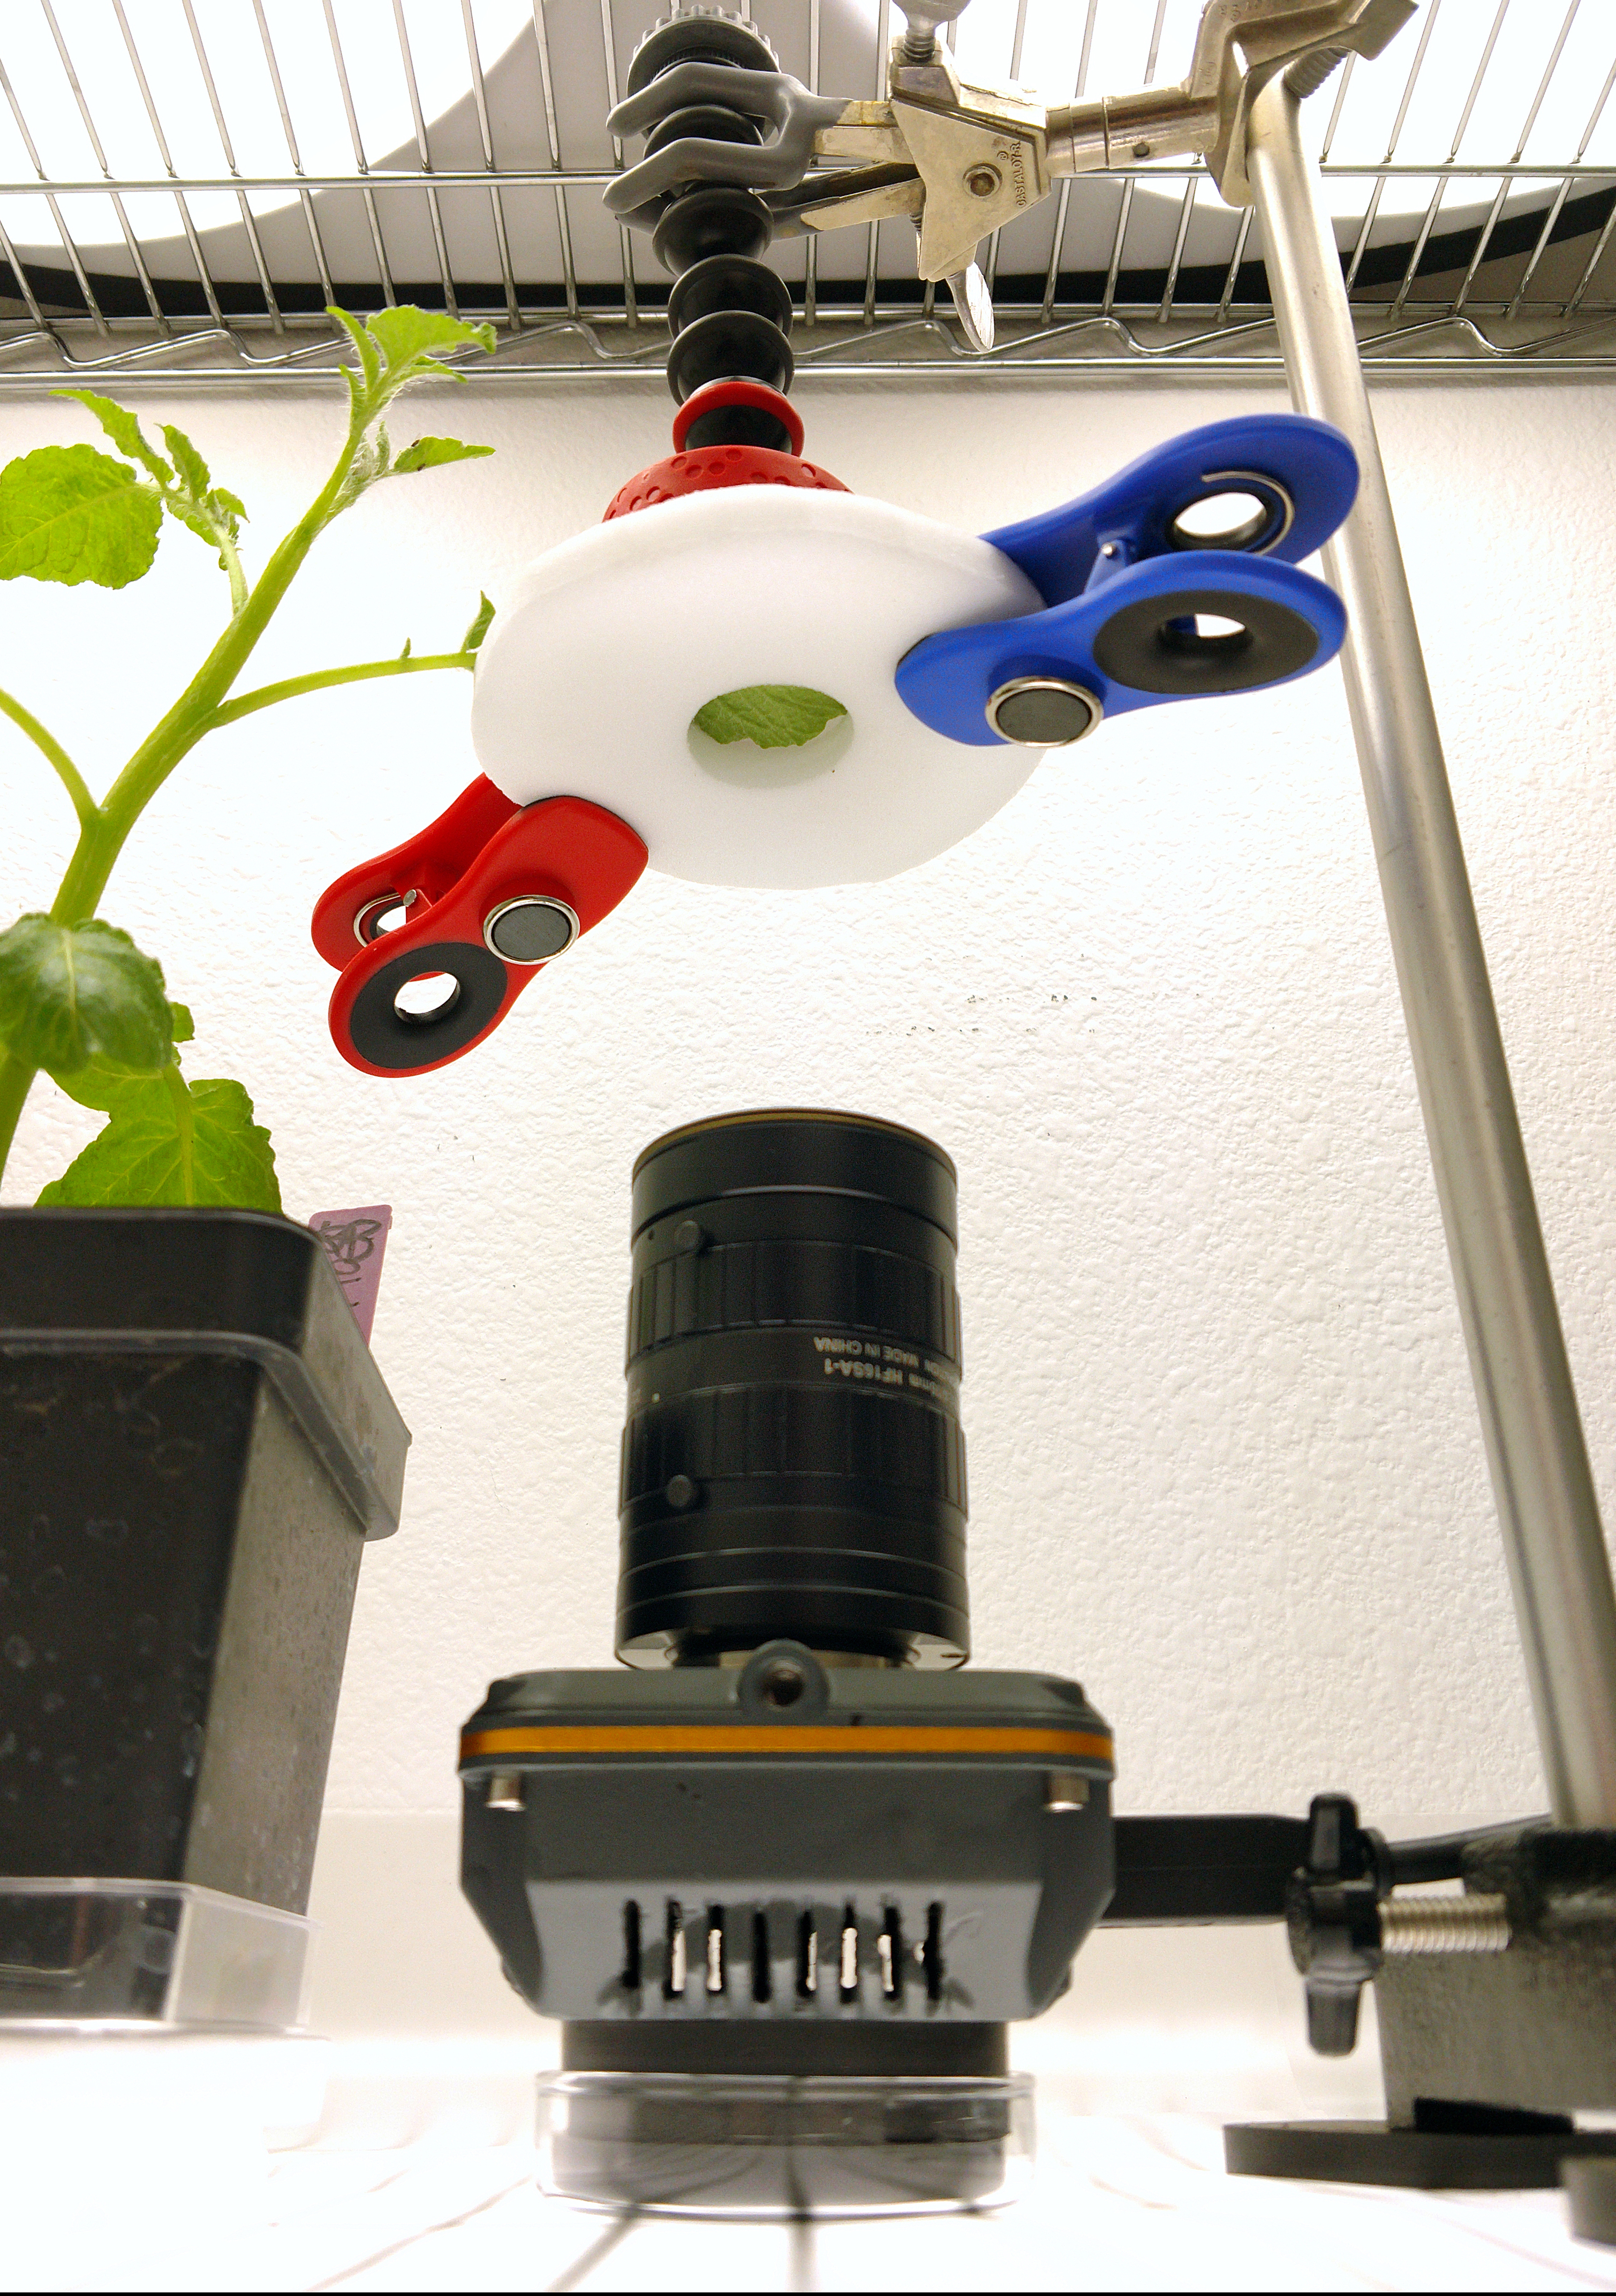
\includegraphics{fig_1.jpg}
\caption{No-choice arena used for behavioral\\
recordings}
\end{figure}

\protect\hypertarget{fig:fig_1}{}{\[fig:fig\_1\]}

\begin{figure}
\centering
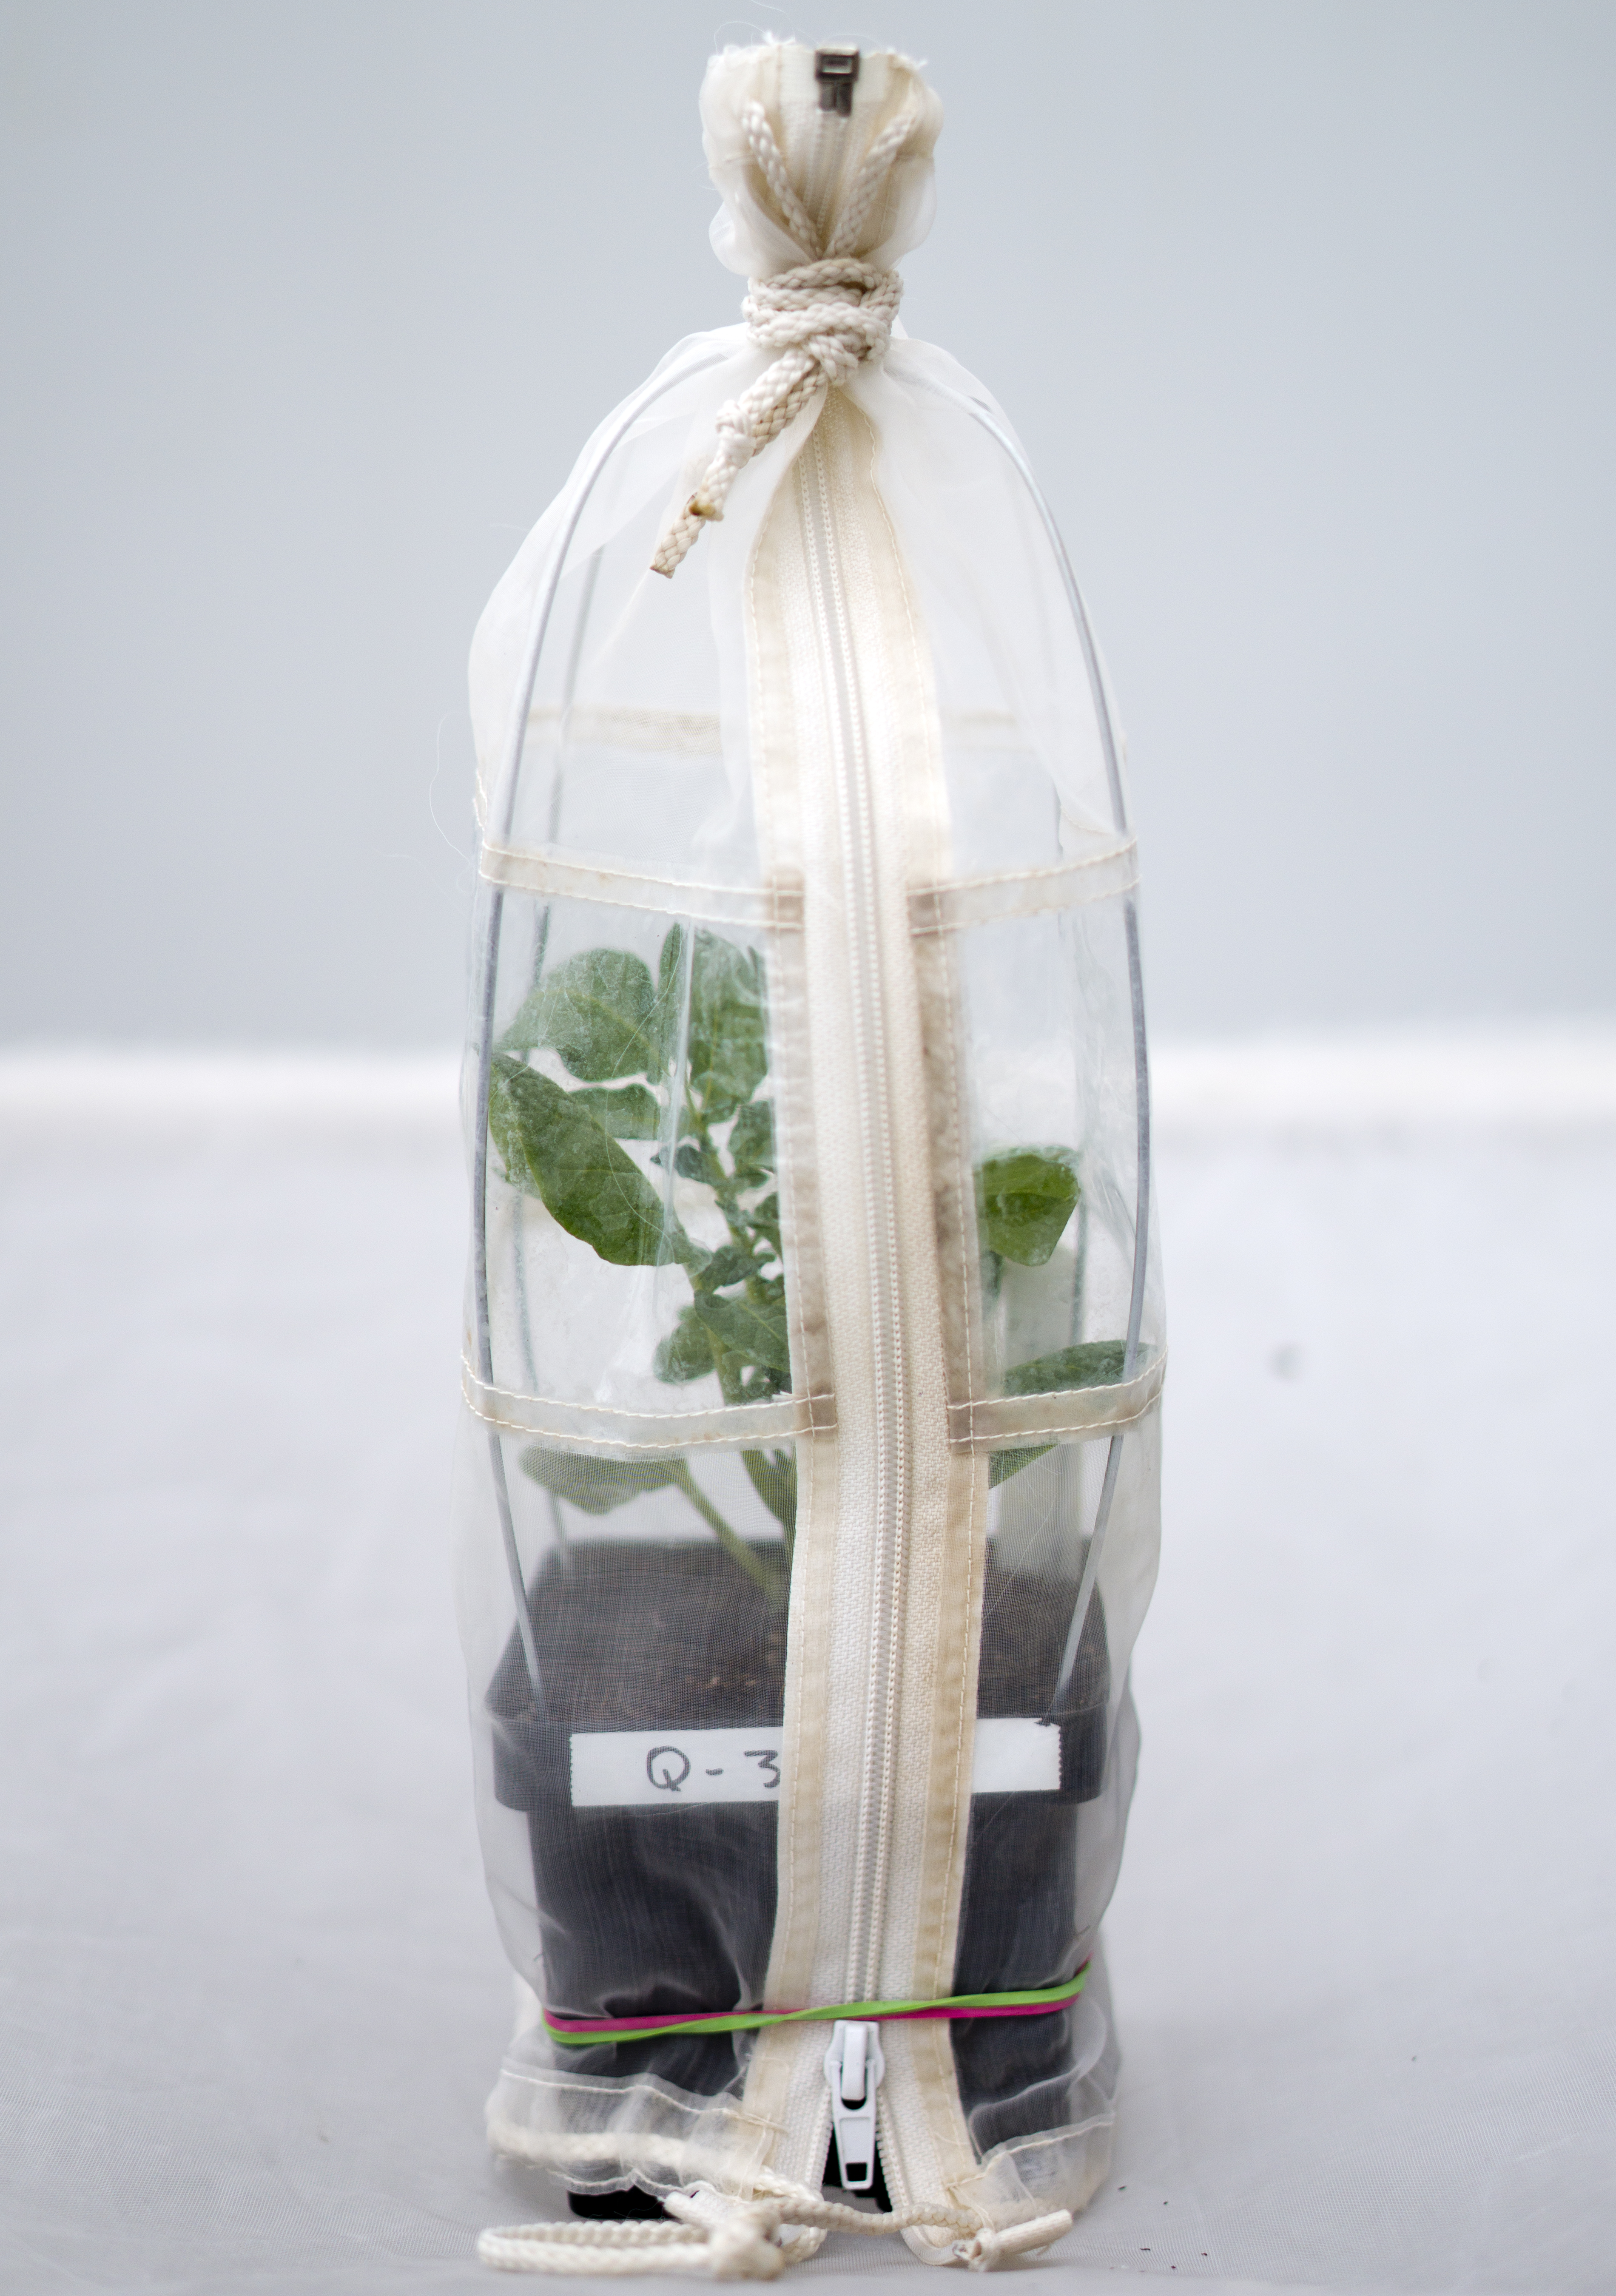
\includegraphics{fig_2.jpg}
\caption{Sleeve cage with potato used in oviposition assays}
\end{figure}

\protect\hypertarget{fig:fig_2}{}{\[fig:fig\_2\]}

\hypertarget{ch:results}{%
\section{Results}\label{ch:results}}

\hypertarget{sec:results_no-choice}{%
\subsection{No-choice assays}\label{sec:results_no-choice}}

The number of probing events observed was significantly different among
genotypes (). Psyllids probed more frequently on Russet Burbank than on
A07781-10LB and A07781-3LB, which did not differ between each other ();
probing frequency on A07781-4LB did not differ among the other
genotypes. This effect appeared to reflect the trend of more probing by
females on Russet Burbank (); however, the genotype \(\times\) sex
interaction was not significant (). Probing frequency did not was not
affected by sex (). Overall, psyllids spent more time engaged in probing
behavior than in the other activities recorded (Tables
\protect\hyperlink{tab:tbl_probes}{\[tab:tbl\_probes\]}-5); however,
probing duration did not differ among genotypes, between sexes or by
their interaction ().

The number of walking events differed significantly among genotypes as
well as by the interaction of genotype \(\times\) sex (). Psyllids
walked more on Russet Burbank than 10LB (). Female psyllids on Russet
Burbank walked significantly more often than males and females on 10LB
and females on 3LB (). The other means did not differ among each other.
Walking duration did not differ among genotypes or between sexes, but
the interaction term was significant (). Female psyllids walked
significantly longer on Russet Burbank than for all other genotype
\(\times\) sex combinations ().

Cleaning behaviors generally were uncommon and of short duration. The
frequencies and durations of cleaning behaviors were not significantly
different among genotypes, betweeen sexes, or in their interaction terms
(, ).

Off-leaf behaviors also tended to occur rarely. Frequency of off-leaf
behaviors did not differ among genotypes, betweeen sexes or by their
interaction (). However, the duration of off-leaf behaviors differed
significantly among genotypes (). Psyllids spent more time off-leaf in
the 3LB treatment relative to the 4LB and Russet Burbank treatments;
time spent off-leaf in the 10LB treatment did not differ among the other
genotypes (). Off-leaf duration did not differ by sex (). The
interaction between genotype and sex could not be analyzed due to the
low number psyllids observed leaving the leaf (n = 20 out of 181).

\hypertarget{sec:results_fecund}{%
\subsection{Oviposition assays}\label{sec:results_fecund}}

Neither the number of eggs laid nor percent viable eggs differed
significantly among genotypes (). However, both the number of eggs laid
and egg fertility were significantly different by period and the
interaction of genotype \(\times\) period (). For oviposition, this
interaction effect was an artifact of calculating multiple comparisons
of different genotypes across observation periods; there were no
significant differences among genotypes within a given period (). For
egg fertility during the last period, there were significantly more
fertile eggs on Russet Burbank than 10LB or 3LB and there were
significantly more eggs on 4LB than 10LB (). There were no significant
differences among genotypes within periods 1-3 (). Overall oviposition
(with genotype pooled) was significantly lower during period 4 than for
the first (). Similarly, egg fertility (with genotype pooled) tended to
decline during the last observation period for all genotype except for
Russet Burbank ().

\hypertarget{ch:discuss}{%
\section{Discussion}\label{ch:discuss}}

It is difficult to separate the mechanisms of host plant resistance or
tolerance and how they to correlate with psyllid host acceptance
(Diaz-Montano et al. \protect\hyperlink{ref-Diaz-Montano2006}{2006},
Butler et al. \protect\hyperlink{ref-Butler2011}{2011}). Furthermore,
visual observation of settling behavior lacks the precision of
electrical penetration recordings used in similar studies Butler et al.
(\protect\hyperlink{ref-Butler2012b}{2012}, Sandanayaka et al.
\protect\hyperlink{ref-Sandanayaka2014}{2014}, Mustafa et al.
\protect\hyperlink{ref-Mustafa2015b}{2015}). Nevertheless, the results
presented here were comparable with similar investigations of putatively
resistant potato genotypes. Our study found more probing and walking on
Russet Burbank than on the putatively resistant genotypes, which is
consistent with results reported by Butler et al.
(\protect\hyperlink{ref-Butler2011}{2011}) and Prager et al.
(\protect\hyperlink{ref-Prager2014b}{2014}, b). However, in contrast to
Butler et al. (\protect\hyperlink{ref-Butler2011}{2011}), we found
cleaning and leaf-leaving behaviors to be rare. Although Russet Burbank
received more probes than two other genotypes, the psyllids still probed
the other genotypes, often for long periods. Sandanayaka et al.
(\protect\hyperlink{ref-Sandanayaka2014}{2014}, and Mustafa et al
\protect\hyperlink{ref-Mustafa2015b}{2015}, b) both suggest that it
takes \emph{B. cockerelli} approximately two hours to access the phloem
and acquire Lso. This suggests that very long recordings may be
necessary to determine when probing becomes true feeding. Minimal
overnight recordings revealed little activity besides apparent feeding
on the genotype where they were placed (ANF, unpublished data). A single
psyllid is enough to transmit Lso and the disease progresses
independently of bacterial titer (Buchman et al.
\protect\hyperlink{ref-Buchman2011a}{2011}, a, Rashed et al.
\protect\hyperlink{ref-Rashed2012}{2012}). Therefore, it is unlikely
that we were observing phloem feeding that would result in pathogen
transmission within the span of our short observation periods. These
factors underscore that psyllid probing behavior would have to be nearly
eliminated to truly reduce the risk of Lso transmission. We found no
evidence for such reductions in probing behavior on these genotypes. A
possible explanation for the higher probing and walking frequencies
observed is that some phytoplasmas (including Lso) can alter psyllid
attraction to leaf volatiles (Mayer et al.
\protect\hyperlink{ref-Mayer2008}{2008}) and affect settling behavior
(Mas et al. \protect\hyperlink{ref-Mas2014}{2014}). The psyllids used in
our experiment were taken from a Lso-positive colony with a high
percentage of infected psyllids. Lso-infected psyllids have increased
preferences for undamaged, uninfected hosts for oviposition and settling
(Davis et al. \protect\hyperlink{ref-Davis2012}{2012}) -- a behavior
which has been seen in other insect-plant-vector relationships (Cao et
al. \protect\hyperlink{ref-Cao2016}{2016}, Eigenbrode et al.
\protect\hyperlink{ref-Eigenbrode2018}{2018}). However, such phenomena
likely do not fully explain the patterns observed here because all
observations in our experiments featured likely Lso-positive psyllids on
Lso-negative plants, regardless of genotype. Studies on the Asian citrus
psyllid, \emph{Diaphorina citri} Kuwayama (Hemiptera: Liviidae), a
vector of other liberibacter pathogens (Teixeira et al.
\protect\hyperlink{ref-Teixeira2005}{2005}) have examined how host plant
volatiles can alter psyllid behavior (Wenninger et al.
\protect\hyperlink{ref-Wenninger2009}{2009}, Davidson et al.
\protect\hyperlink{ref-Davidson2014}{2014}), including increased probing
in response to visual and chemical cues from host plants (Patt et al.
\protect\hyperlink{ref-Patt2011}{2011}). This is a possible explanation
for the minor trend we saw with female psyllids probing more often than
male psyllids. Given that Russet Burbank was the natal plant host from
our colonies, it is possible that the volatiles from this variety were
more stimulating, especially for female psyllids, which may be more
influenced by familiar cues while selecting host plants for oviposition
or feeding Prager et al. (\protect\hyperlink{ref-Prager2014a}{2014}).
Further studies into volatile attractiveness in potato psyllids would
help to clarify how these results relate with host plant acceptance.
Although leaf-leaving duration differed statistically significant among
genotypes, the incidence and duration of leaf-leaving behaviors was very
small and probably not biologically significant. It is also important to
note that leaf-leaving was defined in the context of our observation
arena. On a plant in the field there is a much larger surface area for a
psyllid to explore, so the leaf-leaving events might represent questing
behavior rather than host rejection. It also is possible that the
duration between a psyllid's initial encounter and settling behaviors or
eventual plant rejection is longer than the time we allotted for
recording.

Contrary to previously published studies (Butler et al.
\protect\hyperlink{ref-Butler2011}{2011}, Diaz-Montano et al.
\protect\hyperlink{ref-Diaz-Montano2013}{2013}, Cooper and Bamberg
\protect\hyperlink{ref-Cooper2014}{2014}, Rubio-Covarrubias et al.
\protect\hyperlink{ref-Rubio-Covarrubias2017}{2017}) our study showed
similar oviposition rates among genotypes, consistent with results
reported by (Prager et al. \protect\hyperlink{ref-Prager2017}{2017}).
Other studies have found psyllids will oviposit on a variety of hosts
(Diaz-Montano et al. \protect\hyperlink{ref-Diaz-Montano2013}{2013},
Thinakaran et al. \protect\hyperlink{ref-Thinakaran2015}{2015}), even
when it is not beneficial for their survival (Prager, Lewis, et al.
(\protect\hyperlink{ref-Prager2014b}{2014}) b). Psyllids oviposited on
every type of potato offered, similar to observations by Prager et al.
(\protect\hyperlink{ref-Prager2017}{2017}), giving little evidence of
antixenosis.

We selected the number of days for our observations to correlate with
the periods of maximum oviposition reported in the life history tables
of Abdullah (Knowlton and Janes
\protect\hyperlink{ref-Knowlton1931}{1931},
\protect\hyperlink{ref-Abdullah2008}{2008}, and Yang et al.
\protect\hyperlink{ref-Yang2010}{2010},
\protect\hyperlink{ref-Yang2013}{2013}). Therefore, it was surprising to
see the large reduction of egg fertility for some psyllids in period
four (18-24 days). Fertility declined on the resistant genotypes as
opposed to the Russet Burbank variety, which suggests that these
genotypes may have antibiotic effects over time. Over the course of a
growing season, these reductions may have a cumulative effect on psyllid
populations. Longer observation periods could help to better quantify
these effects.

It is possible that Lso infection status played a role in the fertility
observed: Lso has been reported to negatively impact female fertility
(\protect\hyperlink{ref-Nachappa2012a}{2012} a, Nachappa, Shapiro, et
al. \protect\hyperlink{ref-Nachappa2012}{2012},
\protect\hyperlink{ref-Nachappa2014}{2014}, Yao et al.
\protect\hyperlink{ref-Yao2016}{2016}, Frias et al.
\protect\hyperlink{ref-Frias2018}{2018}). The antibiotic effects we
observed may have different effects on uninfected psyllids.

We saw a large degree of variability in fertility for psyllids on all
genotypes. We only permitted male access to the female psyllids during
the initial period to increase female longevity by preventing possible
harassment (Abdullah \protect\hyperlink{ref-Abdullah2008}{2008},
Wenninger and Hall \protect\hyperlink{ref-Wenninger2008}{2008}, Arnqvist
\protect\hyperlink{ref-Arnqvist2013}{2013}). Abdullah
(\protect\hyperlink{ref-Abdullah2008}{2008}, and Yang and Liu
\protect\hyperlink{ref-Yang2009}{2009}, and Yang et al.
\protect\hyperlink{ref-Yang2013}{2013}) all kept female and male
psyllids together to freely mate for the duration their observations,
which may explain why they observed greater fertility than we did. It is
possible that potato psyllids may require multiple mates and/or multiple
matings over time to maintain egg fertility (Wenninger and Hall
\protect\hyperlink{ref-Wenninger2008}{2008}, Arnqvist
\protect\hyperlink{ref-Arnqvist2013}{2013}). Knowlton and Janes
(\protect\hyperlink{ref-Knowlton1931}{1931}) reported (with a limited
number of observations) reductions in egg fertility over time after a
single mating. There also may be some variability in female reproductive
output created by physiological interactions of male spermatophores,
female spermathecae and/or spermatodose (Marchini et al.
\protect\hyperlink{ref-Marchini2011}{2011}) formation, which influence
how long females are able to remain fertile (Qazi and Hogdal
\protect\hyperlink{ref-Qazi2010}{2010}, Schnakenberg et al.
\protect\hyperlink{ref-Schnakenberg2011}{2011}, Wolfner
\protect\hyperlink{ref-Wolfner2011}{2011}, Abe and Kamimura
\protect\hyperlink{ref-Abe2015}{2015}).

In conclusion, we found little evidence of antixenosis or antibiosis
with respect to settling behavior, but we saw a reduction in egg
fertility on the resistant genotypes 18-24 days after mating. Taken
together, these results suggest that the modality of resistance to Lso
for the A07781 genotypes (Rashidi et al.
\protect\hyperlink{ref-Rashidi2017}{2017}) is not likely related to
psyllid settling behaviors, but that reduced Lso symptoms may be due to
resistance to the pathogen itself, and not the psyllid vector. Further
work will be required to clarify the modality of resistance to Lso in
the A07781 genotypes.

\hypertarget{ch:tables}{%
\section{Tables}\label{ch:tables}}

\protect\hypertarget{tab:tbl_aov}{}{\[tab:tbl\_aov\]}

l S\[table-format=2.2\] S\[table-format=1.0\] S\[table-format=1.3,
table-space-text-post = $^{*}$\] S\[table-format=1.2\]
S\[table-format=1.0\] S\[table-format=1.3, table-space-text-post =
$^{*}$\] \textbf{Behavior} \& \&\\
(l)1-1 (l)2-4 (l)5-7 Factors \& \({\chi^2}\) \& df \& \(\Pr>\chi^2\) \&
\({\chi^2}\) \& df \& \(\Pr>\chi^2\)\\
~\\
~\\
~\\
Genotype \& 27.46 \& 3 \& 0.000\(^{*}\) \& 2.51 \& 3 \& 0.473\\
Sex \& 3.24 \& 1 \& 0.072 \& 0.00 \& 1 \& 0.959\\
Genotype \(\times\) Sex \& 6.49 \& 3 \& 0.090 \& 4.74 \& 3 \& 0.192\\
~\\
~\\
~\\
Genotype \& 16.17 \& 3 \& 0.001\(^{*}\) \& 4.66 \& 3 \& 0.199\\
Sex \& 1.65 \& 1 \& 0.200 \& 0.036 \& 1 \& 0.850\\
Genotype \(\times\) Sex \& 11.13 \& 3 \& 0.011\(^{*}\) \& 10.73 \& 3 \&
0.013\(^{*}\)\\
~\\
~\\
~\\
Genotype \& 5.98 \& 3 \& 0.113 \& 2.23 \& 3 \& 0.525\\
Sex \& 0.45 \& 1 \& 0.503 \& 0.48 \& 1 \& 0.490\\
Genotype \(\times\) Sex \& 0.33 \& 3 \& 0.955 \& 0.09 \& 3 \& 0.993\\
~\\
~\\
~\\
Genotype \& 1.15 \& 3 \& 0.765 \& 2.23 \& 3 \& 0.023\(^{*}\)\\
Sex \& 0.71 \& 1 \& 0.401 \& 0.48 \& 1 \& 0.832\\
Genotype \(\times\) Sex \& --- \& --- \& --- \& --- \& --- \& ---\\
~\\

\(^{*}\) indicates values which are significant at P \textgreater{}
0.05\\
The interaction genotype \(\times\) sex was unable to be analyzed due to
the low number of psyllids which left the leaf (n = 20 out of 181)

\protect\hypertarget{tab:tbl_probes}{}{\[tab:tbl\_probes\]}

r c S\[table-format= \<1.2(2),table-space-text-post= a\] l
S\[table-format= \<3.2(2), add-integer-zero=false,
table-space-text-post= a\] l \textbf{Probing} \&\& Incidence \&\&
Duration (s)\\
Genotype \& N \& Mean\({}\pm{}\)SEM \&\& Mean\({}\pm{}\)SEM\\
~\\
\& 21 \& 1.4 0.26 \& \& 182 28.2 \&\\
\& 25 \& 1.3 0.23 \&\& 242 34.0 \&\\
~\\
\& 27 \& 1.5 0.24 \& \& 248 33.6 \&\\
\& 21 \& 1.4 0.26 \&\& 183 28.2 \&\\
~\\
\& 25 \& 1.7 0.27 \& \& 244 34.1 \&\\
\& 18 \& 1.9 0.34 \&\& 215 35.6 \&\\
~\\
\& 26 \& 3.4 0.38 \& \& 250 34.4 \&\\
\& 18 \& 1.8 0.32 \&\& 285 47.0 \&\\

Least-squares means. Means in the same column which share a letter are
not significantly different (P \textgreater{} 0.05)\\

\protect\hypertarget{tab:tbl_walks}{}{\[tab:tbl\_walks\]}

r c S\[table-format= \<1.2(2),table-space-text-post= a\] l
S\[table-format= \<1.2(2), add-integer-zero=false,
table-space-text-post= a\] l \textbf{Walking} \&\& Incidence \&\&
Duration (s)\\
Genotype \& N \& Mean\({}\pm{}\)SEM \&\& Mean\({}\pm{}\)SEM\\
~\\
\& 21 \& 0.7 0.19 ~\textbf{a} \& \& 0.9 0.8 ~\textbf{a}\\
\& 25 \& 0.3 0.12 ~\textbf{a} \&\& 0.6 0.5 ~\textbf{a}\\
~\\
\& 27 \& 0.5 0.15 ~\textbf{a} \& \& 0.4 0.4 ~\textbf{a}\\
\& 21 \& 0.8 0.21 ~\textbf{ab} \&\& 4.0 3.3 ~\textbf{a}\\
~\\
\& 25 \& 0.9 0.21 ~\textbf{ab} \& \& 1.6 1.3 ~\textbf{a}\\
\& 18 \& 1.1 0.28 ~\textbf{ab} \&\& 5.7 5.0 ~\textbf{a}\\
~\\
\& 26 \& 1.8 0.33 ~\textbf{b} \& \& 10.5 7.5 ~\textbf{b}\\
\& 18 \& 0.6 0.20 ~\textbf{ab} \&\& 0.6 0.6 ~\textbf{a}\\

Least-squares means. Means in the same column which share a letter are
not significantly different (P \textgreater{} 0.05)\\

\protect\hypertarget{tab:tbl_cleans}{}{\[tab:tbl\_cleans\]}

r c S\[table-format= \<1.2(2),table-space-text-post= a\] l
S\[table-format= \<1.3(3), add-integer-zero=false,
table-space-text-post= a\] l \&\& Incidence \&\& Duration (s)\\
Genotype \& N \& Mean\({}\pm{}\)SEM \&\& Mean\({}\pm{}\)SEM\\
~\\
\& 21 \& 0.34 0.15 \&\& 0.008 0.017\\
\& 25 \& 0.33 0.13 \&\& 0.023 0.048\\
~\\
\& 27 \& 0.13 0.07 \&\& 0.002 0.003\\
\& 21 \& 0.20 0.10 \&\& 0.003 0.005\\
~\\
\& 25 \& 0.20 0.10 \&\& 0.002 0.003\\
\& 18 \& 0.26 0.13 \&\& 0.008 0.018\\
~\\
\& 26 \& 0.09 0.05 \&\& 0.001 0.001\\
\& 18 \& 0.13 0.08 \&\& 0.001 0.002\\

Least-squares means. Means in the same column which share a letter are
not significantly different (P \textgreater{} 0.05)\\

\protect\hypertarget{tab:tbl_off}{}{\[tab:tbl\_off\]}

r c S\[table-format= \<1.2(2),table-space-text-post= a\] l
S\[table-format= \<4.1(5), add-integer-zero=false,
table-space-text-post= a\] l l l \&\& Incidence \&\& Duration (s)\\
Genotype \& N \& Mean\({}\pm{}\)SEM \&\& Mean\({}\pm{}\)SEM\\
~\\
\& 21 \& 0.03 0.02 \&\& 1449.9 2934.1 \({\times}\) 10\(^{-7}\) \&\&\&\\
\& 25 \& 0.05 0.03 \&\& 1873.6 3716.9 \({\times}\) 10\(^{-7}\)\\
~\\
\& 27 \& 0.06 0.03 \&\& 2229.5 4272.9 \({\times}\) 10\(^{-7}\) \&\&\&\\
\& 21 \& 0.09 0.05 \&\& 2881.0 5700.0 \({\times}\) 10\(^{-7}\)\\
~\\
\& 25 \& 0.05 0.04 \&\& 10.6 31.6 \({\times}\) 10\(^{-7}\) \&\&\&\\
\& 18 \& 0.08 0.06 \&\& 13.7 41.6 \({\times}\) 10\(^{-7}\)\\
~\\
\& 26 \& 0.03 0.02 \&\& 9.1 27.1 \({\times}\) 10\(^{-7}\) \&\&\&\\
\& 18 \& 0.05 0.03 \&\& 11.7 35.7 \({\times}\) 10\(^{-7}\)\\

Least-squares means. Means in the same column which share a letter are
not significantly different (P \textgreater{} 0.05)\\

\({^\ddagger}\) Off-leaf interactions were unable to be analyzed
statistically due to low numbers of replicates (n = 20 out of 181).

\protect\hypertarget{tab:tbl_fcnd_aov}{}{\[tab:tbl\_fcnd\_aov\]}

l S\[table-format=2.2\] S\[table-format=1.0\] S\[table-format=1.3,
table-space-text-post = $^{*}$\] S\[table-format=1.2\]
S\[table-format=1.0\] S\[table-format=1.3, table-space-text-post =
$^{*}$\] \& \&\\
Factors \& \({\chi^2}\) \& df \& \(\Pr>\chi^2\) \& \({\chi^2}\) \& df \&
\(\Pr>\chi^2\)\\
~\\
Genotype \& 0.84 \& 3 \& 0.84 \& 0.21 \& 3 \& 0.976\\
Period \& 70.23 \& 3 \& 0.000\(^{*}\) \& 25.60 \& 3 \& 0.000\(^{*}\)\\
Genotype \({\times}\) Period \& 51.00 \& 9 \& 0.000\(^{*}\) \& 81.93 \&
9 \& 0.000\(^{*}\)\\
~\\

center

\protect\hypertarget{tab:tbl_fcnd}{}{\[tab:tbl\_fcnd\]}

l c S\[table-format=1.2(2),table-space-text-post= a\]
S\[table-format=1.2(2),table-space-text-post= a\]
S\[table-format=1.2(2),table-space-text-post= a\]
S\[table-format=1.2(2),table-space-text-post= a\] \& \textbf{N} \& \& \&
\&\\
~\\
10LB \& \textbf{20} \& 6.3 1.5 \& 7.0 1.7 \& 9.4 2.3\& 3.8 1.0\\
3LB \& \textbf{13} \& 4.8 1.4 \& 9.5 2.8 \& 9.1 2.7 \& 4.3 1.3\\
4LB \& \textbf{19} \& 8.4 2.0 \& 10.5 2.6 \& 8.0 2.0 \& 6.9 1.8\\
Russet Burbank \& \textbf{14} \& 5.8 1.7 \& 7.6 2.2 \& 7.0 2.0 \& 6.6
1.9\\
Overall\(^\dagger\) \& \textbf{66} \& 9.5 1.6 \& 12.5 1.8 \& 12.5 2.0 \&
8.2 1.5\\
~\\
\textbf{Percent Fertile}\\
~\\
10LB \&\& 68.8 9.2 ~\& 59.5 10.9 ~\& 61.8 10.7 ~\& 3.2 2.0 ~\textbf{a}\\
3LB \&\& 65.9 12.8 ~\& 61.0 12.6 ~\& 55.7 13.3 ~\& 11.9 6.8
~\textbf{ab}\\
4LB \&\& 62.3 10.5 ~\& 64.1 10.1 ~\& 49.6 12.2 ~\& 29.2 10.4
~\textbf{bc}\\
Russet Burbank \&\& 47.0 13.0 ~\& 50.9 12.7 ~\& 63.9 11.9 ~\& 70.1 10.9
~\textbf{c}\\
Overall\(^\dagger\) \& \textbf{66} \& 66.8 4.2 \textbf{a} \& 68.2 4.0
\textbf{ab} \& 66.0 5.5 \textbf{ab} \& 43.8 6.2 \textbf{b}\\
~\\

\(^\dagger\) Letters represent differences among periods (\emph{P}
\textgreater{} 0.05)

Means in the same column which share a letter are not significantly
different (\emph{P} \textgreater{} 0.05)\\

\hypertarget{refs}{}
\leavevmode\hypertarget{ref-Abdullah2008}{}%
\textbf{Abdullah, N. M. H.} \textbf{2008}. Life history of the potato
psyllid \emph{bactericera cockerelli} (homoptera: Psyllidae) in
controlled environments agriculture in arizona. Afr. J. Agric. Res. 3:
60--67.

\leavevmode\hypertarget{ref-Abe2015}{}%
\textbf{Abe, J., and Y. Kamimura}. \textbf{2015}. Sperm economy between
female mating frequency and male ejaculate allocation. The American
Naturalist. 185: 406--416.

\leavevmode\hypertarget{ref-Aguilar2013}{}%
\textbf{Aguilar, E., V. G. Sengoda, B. Bextine, K. F. McCue, and J. E.
Munyaneza}. \textbf{2013}. First report of "\emph{candidatus}
Liberibacter solanacearum" on tobacco in Honduras. Plant Disease. 97:
1376--1376.

\leavevmode\hypertarget{ref-Alvarado2012}{}%
\textbf{Alvarado, V. Y., D. Odokonyero, O. Duncan, T. E. Mirkov, and H.
B. Scholthof}. \textbf{2012}. Molecular and physiological properties
associated with zebra complex disease in potatoes and its relation with
\emph{candidatus} liberibacter contents in psyllid vectors. PLoS ONE. 7:
e37345.

\leavevmode\hypertarget{ref-Anderson2012}{}%
\textbf{Anderson, J. A. D., G. P. Walker, P. A. Alspach, M. Jeram, and
P. J. Wright}. \textbf{2012}. Assessment of susceptibility to zebra chip
and \emph{bactericera cockerelli} of selected potato cultivars under
different insecticide regimes in new zealand. Am. J. Potato Res. 90:
58--65.

\leavevmode\hypertarget{ref-Arnqvist2013}{}%
\textbf{Arnqvist, G.} \textbf{2013}. Sexual conflict. Princeton
University Press.

\leavevmode\hypertarget{ref-Bates2015}{}%
\textbf{Bates, D., M. Mächler, B. Bolker, and S. Walker}. \textbf{2015}.
Fitting linear mixed-effects models using lme4. Journal of statistical
software. 67.

\leavevmode\hypertarget{ref-Buchman2012}{}%
\textbf{Buchman, J. L., T. W. Fisher, V. G. Sengoda, and J. E.
Munyaneza}. \textbf{2012}. Zebra chip progression: From inoculation of
potato plants with liberibacter to development of disease symptoms in
tubers. Am. J. Potato Res. 89: 159--168.

\leavevmode\hypertarget{ref-Buchman2011a}{}%
\textbf{Buchman, J. L., V. G. Sengoda, and J. E. Munyaneza}.
\textbf{2011}. Vector transmission efficiency of liberibacter by
\emph{bactericera cockerelli} (hemiptera: Triozidae) in zebra chip
potato disease: Effects of psyllid life stage and inoculation access
period. J. Econ. Entomol. 104: 1486--1495.

\leavevmode\hypertarget{ref-Butler2011}{}%
\textbf{Butler, C. D., B. Gonzalez, K. L. Manjunath, R. F. Lee, R. G.
Novy, J. C. Miller, and J. T. Trumble}. \textbf{2011}. Behavioral
responses of adult potato psyllid, \emph{bactericera cockerelli}
(hemiptera: Triozidae), to potato germplasm and transmission of
\emph{candidatus} liberibacter psyllaurous. Crop Prot. 30: 1233--1238.

\leavevmode\hypertarget{ref-Butler2012a}{}%
\textbf{Butler, C. D., and J. T. Trumble}. \textbf{2012}. The potato
psyllid, \emph{bactericera cockerelli} (Šulc) (hemiptera: Triozidae):
Life history, relationship to plant diseases, and management strategies.
Terrestrial arthropod reviews. 5: 87--111.

\leavevmode\hypertarget{ref-Butler2012b}{}%
\textbf{Butler, C. D., G. P. Walker, and J. T. Trumble}. \textbf{2012}.
Feeding disruption of potato psyllid, \emph{bactericera cockerelli}, by
imidacloprid as measured by electrical penetration graphs. Entomol. Exp.
Appl. 142: 247--257.

\leavevmode\hypertarget{ref-Cao2016}{}%
\textbf{Cao, H., H. Liu, Z. Zhang, and T. Liu}. \textbf{2016}. The green
peach aphid \emph{myzus persicae} perform better on pre-infested chinese
cabbage \emph{brassica pekinensis} by enhancing host plant nutritional
quality. Sci. Rep. 6.

\leavevmode\hypertarget{ref-Casteel2006}{}%
\textbf{Casteel, C. L., L. L. Walling, and T. D. Paine}. \textbf{2006}.
Behavior and biology of the tomato psyllid, \emph{bactericerca
cockerelli}, in response to the mi-1.2 gene. Entomol. Exp. Appl. 121:
67--72.

\leavevmode\hypertarget{ref-Casteel2007}{}%
\textbf{Casteel, C. L., L. L. Walling, and T. D. Paine}. \textbf{2007}.
Effect of mi-1.2 gene in natal host plants on behavior and biology of
the tomato psyllid \emph{bactericerca cockerelli} (sulc) (hemiptera:
Psyllidae). Journal of Entomological Science. 42: 155--162.

\leavevmode\hypertarget{ref-Chavez2015}{}%
\textbf{Chávez, E. C., O. H. Bautista, J. L. Flores, L. A. Uribe, and Y.
M. O. Fuentes}. \textbf{2015}. Insecticide-resistance ratios of three
populations of \emph{bactericera cockerelli} (hemiptera: Psylloidea:
Triozidae) in regions of northern mexico. Florida Entomologist. 98:
950--953.

\leavevmode\hypertarget{ref-Cicero2016}{}%
\textbf{Cicero, J. M., T. W. Fisher, and J. K. Brown}. \textbf{2016}.
Localization of ``\emph{candidatus} liberibacter solanacearum'' and
evidence for surface appendages in the potato psyllid vector.
Phytopathology. 106: 142--154.

\leavevmode\hypertarget{ref-Cooper2014}{}%
\textbf{Cooper, W. R., and J. B. Bamberg}. \textbf{2014}. Variation in
\emph{bactericera cockerelli} (hemiptera: Triozidae) oviposition,
survival, and development on \emph{solanum bulbocastanum} germplasm. Am.
J. Potato Res. 91: 532--537.

\leavevmode\hypertarget{ref-Crosslin2011}{}%
\textbf{Crosslin, J. M., H. Lin, and J. E. Munyaneza}. \textbf{2011}.
Detection of ``\emph{candidatus} liberibacter solanacearum'' in the
potato psyllid, \emph{bactericera cockerelli} (sulc), by conventional
and real-time PCR. Southwestern Entomologist. 36: 125--135.

\leavevmode\hypertarget{ref-Crosslin2012}{}%
\textbf{Crosslin, J. M., N. Olsen, and P. Nolte}. \textbf{2012}. First
report of zebra chip disease and \emph{candidatus} liberibacter
solanacearum on potatoes in idaho. Plant Dis. 96: 453--453.

\leavevmode\hypertarget{ref-Dahan2017}{}%
\textbf{Dahan, J., E. J. Wenninger, B. Thompson, S. Eid, N. Olsen, and
A. V. Karasev}. \textbf{2017}. Relative abundance of potato psyllid
haplotypes in southern idaho potato fields during 2012 to 2015, and
incidence of ``\emph{candidatus} liberibacter solanacearum'' causing
zebra chip disease. Plant Dis. 101: 822--829.

\leavevmode\hypertarget{ref-Davidson2014}{}%
\textbf{Davidson, M. M., R. C. Butler, N. M. Taylor, M. C. Nielsen, C.
E. Sansom, and N. B. Perry}. \textbf{2014}. A volatile compound,
2-undecanone, increases walking, but not flying, tomato potato psyllid
movement toward an odour source. New Zealand plant protection. 67:
184--190.

\leavevmode\hypertarget{ref-Davis2012}{}%
\textbf{Davis, T. S., D. R. Horton, J. E. Munyaneza, and P. J. Landolt}.
\textbf{2012}. Experimental infection of plants with an
herbivore-associated bacterial endosymbiont influences herbivore host
selection behavior. PLoS ONE. 7: e49330.

\leavevmode\hypertarget{ref-Delignette-Muller2015}{}%
\textbf{Delignette-Muller, M. L., and C. Dutang}. \textbf{2015}.
fitdistrplus: An R package for fitting distributions. Journal of
Statistical Software. 64.

\leavevmode\hypertarget{ref-Diaz-Montano2006}{}%
\textbf{Diaz-Montano, J., J. C. Reese, W. T. Schapaugh, and L. R.
Campbell}. \textbf{2006}. Characterization of antibiosis and antixenosis
to the soybean aphid (hemiptera: Aphididae) in several soybean
genotypes. J. Econ. Entomol. 99: 1884--1889.

\leavevmode\hypertarget{ref-Diaz-Montano2013}{}%
\textbf{Diaz-Montano, J., B. G. Vindiola, N. Drew, R. G. Novy, J. C.
Miller, and J. T. Trumble}. \textbf{2013}. Resistance of selected potato
genotypes to the potato psyllid (hemiptera: Triozidae). Am. J. Potato
Res. 91: 363--367.

\leavevmode\hypertarget{ref-Dwelle2003}{}%
\textbf{Dwelle, R. B., J. M. Alvarez, P. Bain, C. R. Baird, E. J.
Bechinski, W. H. Bohl, D. L. Corsini, C. V. Eberlein, L. L. Ewing, B. F.
Finnigan, B. D. Geary, J. F. Guenthner, S. L. Hafez, P. J. S.
Hutchinson, W. B. Jones, B. A. King, G. E. Kleinkopf, J. S. Miller, P.
Nolte, R. Novy, N. Olsen, S. Palanisamy, P. E. Patterson, L. E. Sandvol,
R. L. Stoltz, D. T. Westermann, and J. C. Whitmore}. \textbf{2003}.
Potato production systems, pp. 12--14. \emph{In}. The University of
Idaho agricultural communications.

\leavevmode\hypertarget{ref-Echegaray2017}{}%
\textbf{Echegaray, E. R., and S. I. Rondon}. \textbf{2017}. Incidence of
\emph{bactericera cockerelli} (hemiptera: Triozidae) under different
pesticide regimes in the lower columbia basin. J. Econ. Entomol. 110:
1639--1647.

\leavevmode\hypertarget{ref-Eigenbrode2018}{}%
\textbf{Eigenbrode, S. D., N. A. Bosque-Pérez, and T. S. Davis}.
\textbf{2018}. Insect-borne plant pathogens and their vectors: Ecology,
evolution, and complex interactions. Annu. Rev. Entomol. 63: 169--191.

\leavevmode\hypertarget{ref-Eyer1933}{}%
\textbf{Eyer, J. R., and R. F. Crawford}. \textbf{1933}. Observations on
the feeding habits of the potato psyllid (\emph{paratrioza cockerelli}
sulc.) and the pathological history of the "psyllid yellows" which it
produces. J. Econ. Entomol. 26: 846--850.

\leavevmode\hypertarget{ref-Frias2018}{}%
\textbf{Frias, A. A. T., F. Ibanez, A. Mendoza, W. M. de Carvalho Nunes,
and C. Tamborindeguy}. \textbf{2018}. Effects of "\emph{candidatus}
Liberibacter solanacearum" (haplotype b) on \emph{bactericera
cockerelli} fitness and vitellogenesis. Insect Science.

\leavevmode\hypertarget{ref-Gharalari2009}{}%
\textbf{Gharalari, A. H., C. Nansen, D. S. Lawson, J. Gilley, J. E.
Munyaneza, and K. Vaughn}. \textbf{2009}. Knockdown mortality,
repellency, and residual effects of insecticides for control of adult
\emph{bactericera cockerelli} (hemiptera: Psyllidae). J. Econ. Entomol.
102: 1032--1038.

\leavevmode\hypertarget{ref-Goolsby2007b}{}%
\textbf{Goolsby, J. A., J. Adamczyk, B. Bextine, D. Lin, J. E.
Munyaneza, and G. Bester}. \textbf{2007}. Development of an ipm program
for management of the potato psyllid to reduce incidence of zebra chip
disorder in potatoes. Subtropical Plant Science. 59: 85--94.

\leavevmode\hypertarget{ref-Goolsby2007a}{}%
\textbf{Goolsby, J. A., B. Bextine, J. E. Munyaneza, M. Setamou, J.
Adamczyk, and G. Bester}. \textbf{2007}. Seasonal abundance of
sharpshooters, leafhoppers, and psyllids associated with potatoes
affected by zebra chip disorder. Subtropical Plant Science. 59: 15--23.

\leavevmode\hypertarget{ref-Greenway2014}{}%
\textbf{Greenway, G.} \textbf{2014}. Economic impact of zebra chip
control costs on grower returns in seven US states. Am. J. Potato Res.
91: 714--719.

\leavevmode\hypertarget{ref-Greenway2018}{}%
\textbf{Greenway, G. A., and S. Rondon}. \textbf{2018}. Economic impacts
of zebra chip in idaho, oregon, and washington. Am. J. Potato Res.

\leavevmode\hypertarget{ref-Guenthner2012}{}%
\textbf{Guenthner, J., J. Goolsby, and G. Greenway}. \textbf{2012}. Use
and cost of insecticides to control potato psyllids and zebra chip on
potatoes. Southwestern Entomologist. 37: 263--270.

\leavevmode\hypertarget{ref-Hansen2008}{}%
\textbf{Hansen, A. K., J. T. Trumble, R. Stouthamer, and T. D. Paine}.
\textbf{2008}. A new huanglongbing species, "\emph{candidatus}
liberibacter psyllaurous," found to infect tomato and potato, is
vectored by the psyllid \emph{(}bactericera cockerelli) (sulc). Appl.
Environ. Microbiol. 74: 5862--5865.

\leavevmode\hypertarget{ref-Haenninen2009}{}%
\textbf{Hänninen, L., and M. Pastell}. \textbf{2009}. CowLog:
Open-source software for coding behaviors from digital video. Behav.
Res. Methods. 41: 472--476.

\leavevmode\hypertarget{ref-Hernandez-Bautista2013}{}%
\textbf{Hernández-Bautista, O., E. Cerna-Chávez, J. Landeros-Flores, Y.
Ochoa-Fuentes, J. Chacón-Hernández, and S. Castillo-Arriaga}.
\textbf{2013}. Resistance proportion of \emph{bactericera cockerelli}
(sulc) in regions from villa de arista, san luis potosí and saltillo,
coahuila. Entomología mexicana.

\leavevmode\hypertarget{ref-Hodkinson2015}{}%
\textbf{Hodkinson, I. D., C. V. Achterberg, M. Ahola, M. Barták, V.
Behan-Pelletier, J. M. Bird, K. Bøg, F. Brodo, P. N. Buhl, C. Dahl, R.
H. L. Disney, K. Dittmar, A. Fjellberg, Ø. Gammelmo, M. Forshage, R.
Gerecke, C. A. Gertsson, M. M. L. Haastriter, J. P. Haenni, O. E. Heie,
J. M. Heraty, C. Hodgson, D. Horsfield, J. T. Huber, M. Jaschoff, F.
Jensen, K. A. Johanson, R. Jussila, O. Karsholt, E. Krzeminska, V. I.
Lantsov, P. Láska, C. Lindegaard, L. Lyneborg, O. Makarova, Y. M.
Marusik, W. N. Mathis, L. Mazánek, V. Michelsen, T. Munk, W. L. Murphy,
S. A. Nielsen, T. R. Nielsen, J. S. Noyes, P. Oosterbroek, A. L. Ozerov,
T. Pape, J. D. Pinto, M. Pollet, E. Rindal, J. Rohácek, T. J. Simonsen,
V. S. Smith, G. Söli, J. Starý, R. Z. Strassen, B. W. Svensson, L.
Vilhelmsen, P. Vilkamaa, M. Wilson, and T. Zatwarnicki}. \textbf{2015}.
Psyllidae (jumping plant-lice, psyllids), p. 113. \emph{In} The
Greenland Entomofauna: An Identification Manual of Insects, Spiders and
Their Allies (Fauna Entomologica Scandinavica). Brill Academic Pub.

\leavevmode\hypertarget{ref-Kaloshian2004}{}%
\textbf{Kaloshian, I.} \textbf{2004}. Gene-for-gene disease resistance:
Bridging insect pest and pathogen defense. J. Chem. Ecol. 30:
2419--2438.

\leavevmode\hypertarget{ref-Kennedy1987}{}%
\textbf{Kennedy, G. G., F. Gould, O. M. B. Deponti, and R. E. Stinner}.
\textbf{1987}. Ecological, agricultural, genetic, and commercial
considerations in the deployment of insect-resistant germplasm. Environ.
Entomol. 16: 327--338.

\leavevmode\hypertarget{ref-Klingler2005}{}%
\textbf{Klingler, J., R. Creasy, L. Gao, R. M. Nair, A. S. Calix, H. S.
Jacob, O. R. Edwards, and K. B. Singh}. \textbf{2005}. Aphid resistance
in \emph{medicago truncatula} involves antixenosis and phloem-specific,
inducible antibiosis, and maps to a single locus flanked by NBS-LRR
resistance gene analogs. Plant Physiol. 137: 1445--1455.

\leavevmode\hypertarget{ref-Knowlton1931}{}%
\textbf{Knowlton, G. F., and M. J. Janes}. \textbf{1931}. Studies on the
biology of \emph{paratrioza cockerelli} (sulc). Ann. Entomol. Soc. Am.
24: 283--292.

\leavevmode\hypertarget{ref-Knowlton1934}{}%
\textbf{Knowlton, G. F., and W. L. Thomas}. \textbf{1934}. Host plants
of the potato psyllid. J. Econ. Entomol. 27: 547--549.

\leavevmode\hypertarget{ref-Kogan1988}{}%
\textbf{Kogan, M.} \textbf{1988}. Integrated pest management theory and
practice. Entomol. Exp. Appl. 49: 59--70.

\leavevmode\hypertarget{ref-Levy2011}{}%
\textbf{Levy, J., A. Ravindran, D. Gross, C. Tamborindeguy, and E.
Pierson}. \textbf{2011}. Translocation of ``\emph{candidatus}
liberibacter solanacearum'', the zebra chip pathogen, in potato and
tomato. Phytopathology. 101: 1285--1291.

\leavevmode\hypertarget{ref-Li2009}{}%
\textbf{Li, W., J. A. Abad, R. D. French-Monar, R. J., A. Wen, N. C.
Gudmestad, G. A. Secor, I. M. Lee, Y. Duan, and L. Levy}. \textbf{2009}.
Multiplex real-time PCR for detection, identification and quantification
of ``\emph{candidatus} liberibacter solanacearum'' in potato plants with
zebra chip. J. Microbiol. Methods. 78: 59--65.

\leavevmode\hypertarget{ref-Li2006}{}%
\textbf{Li, W., J. S. Hartung, and L. Levy}. \textbf{2006}. Quantitative
real-time PCR for detection and identification of \emph{candidatus}
liberibacter species associated with citrus huanglongbing. J. Microbiol.
Methods. 66: 104--115.

\leavevmode\hypertarget{ref-Liefting2008}{}%
\textbf{Liefting, L. W., L. I. Ward, J. B. Shiller, and G. R. G.
Clover}. \textbf{2008}. A new ``\emph{candidatus} liberibacter'' species
in \emph{solanum betaceum} (tamarillo) and \emph{physalis peruviana}
(cape gooseberry) in new zealand. Plant Dis. 92: 1588--1588.

\leavevmode\hypertarget{ref-Liefting2009}{}%
\textbf{Liefting, L. W., B. S. Weir, S. R. Pennycook, and G. R. G.
Clover}. \textbf{2009}. '\emph{Candidatus} liberibacter solanacearum',
associated with plants in the family solanaceae. Int. J. Syst. Evol.
Microbiol. 59: 2274--2276.

\leavevmode\hypertarget{ref-Lin2009}{}%
\textbf{Lin, H., H. Doddapaneni, J. E. Munyaneza, E. L. Civerolo, V. G.
Sengoda, J. L. Buchman, and D. C. Stenger}. \textbf{2009}. Molecular
characterization and phylogenetic analysis of 16S rRNA from a new
"\emph{candidatus} liberibacter" strain associated with zebra chip
disease of potato (\emph{solanum tuberosum} l.) and the potato psyllid
(\emph{bactericera cockerelli} sulc). Journal of plant pathology. 91:
215--219.

\leavevmode\hypertarget{ref-Liu2004}{}%
\textbf{Liu, D., and J. T. Trumble}. \textbf{2004}. Tomato psyllid
behavioral responses to tomato plant lines and interactions of plant
lines with insecticides. J. Econ. Entomol. 97: 1078--1085.

\leavevmode\hypertarget{ref-Marchini2011}{}%
\textbf{Marchini, D., G. D. Bene, R. Viscuso, and R. Dallai}.
\textbf{2011}. Sperm storage by spermatodoses in the spermatheca of
\emph{trioza alacris} (flor, 1861) hemiptera, psylloidea, triozidae: A
structural and ultrastructural study. J. Morphol. 273: 195--210.

\leavevmode\hypertarget{ref-Martin2008}{}%
\textbf{Martin, N. A.} \textbf{2008}. Host plants of the potato/tomato
psyllid: A cautionary tale. The Weta. 35: 12--16.

\leavevmode\hypertarget{ref-Marzachi1998}{}%
\textbf{Marzachi, C., F. Beratti, and D. Bosco}. \textbf{1998}. Direct
PCR detection of phytoplasmas in experimentally infected insects. Ann.
Appl. Biol. 133: 45--54.

\leavevmode\hypertarget{ref-Mas2014}{}%
\textbf{Mas, F., J. Vereijssen, and D. M. Suckling}. \textbf{2014}.
Influence of the pathogen \emph{candidatus} liberibacter solanacearum on
tomato host plant volatiles and psyllid vector settlement. J. Chem.
Ecol. 40: 1197--1202.

\leavevmode\hypertarget{ref-Mayer2008}{}%
\textbf{Mayer, C. J., A. Vilcinskas, and J. Gross}. \textbf{2008}.
Phytopathogen lures its insect vector by altering host plant odor. J.
Chem. Ecol. 34: 1045--1049.

\leavevmode\hypertarget{ref-Munyaneza2012b}{}%
\textbf{Munyaneza, J. E.} \textbf{2012}. Zebra chip disease of potato:
Biology, epidemiology, and management. Am. J. Potato Res. 89: 329--350.

\leavevmode\hypertarget{ref-Munyaneza2011}{}%
\textbf{Munyaneza, J. E., J. L. Buchman, V. G. Sengoda, T. W. Fisher,
and C. C. Pearson}. \textbf{2011}. Susceptibility of selected potato
varieties to zebra chip potato disease. Am. J. Potato Res. 88: 435--440.

\leavevmode\hypertarget{ref-Munyaneza2008}{}%
\textbf{Munyaneza, J. E., J. L. Buchman, J. E. Upton, J. A. Goolsby, J.
M. Crosslin, G. Bester, G. P. Miles, and V. G. Sengoda}. \textbf{2008}.
Main content area impact of different potato psyllid populations on
zebra chip disease incidence, severity, and potato yield. Subtropical
plant science. 60: 27--37.

\leavevmode\hypertarget{ref-Munyaneza2007a}{}%
\textbf{Munyaneza, J. E., J. M. Crosslin, and J. E. Upton}.
\textbf{2007}. Association of \emph{bactericera cockerelli} (homoptera:
Psyllidae) with 'zebra chip,' a new potato disease in southwestern
united states and mexico. J. Econ. Entomol. 100: 656--663.

\leavevmode\hypertarget{ref-Munyaneza2009}{}%
\textbf{Munyaneza, J. E., V. G. Sengoda, J. M. Crosslin, G. D. la
Rosa-Lozano, and A. Sanchez}. \textbf{2009}. First report of
``\emph{candidatus} liberibacter psyllaurous'' in potato tubers with
zebra chip disease in mexico. Plant Dis. 93: 552--552.

\leavevmode\hypertarget{ref-Murphy2012}{}%
\textbf{Murphy, A. F., S. I. Rondon, and A. S. Jensen}. \textbf{2012}.
First report of potato psyllids, \emph{bactericera cockerelli},
overwintering in the pacific northwest. Am. J. Potato Res. 90: 294--296.

\leavevmode\hypertarget{ref-Mustafa2015b}{}%
\textbf{Mustafa, T., D. R. Horton, W. R. Cooper, K. D. Swisher, R. S.
Zack, H. R. Pappu, and J. E. Munyaneza}. \textbf{2015}. Use of
electrical penetration graph technology to examine transmission of
``\emph{candidatus} liberibacter solanacearum'' to potato by three
haplotypes of potato psyllid (\emph{bactericera cockerelli}; (hemiptera:
Triozidae). PLoS ONE. 10: e0138946.

\leavevmode\hypertarget{ref-Nachappa2012a}{}%
\textbf{Nachappa, P., J. Levy, and C. Tamborindeguy}. \textbf{2012}.
Transcriptome analyses of \emph{bactericera cockerelli} adults in
response to "\emph{candidatus} Liberibacter solanacearum" infection.
Molecular genetics and genomics. 287: 803--817.

\leavevmode\hypertarget{ref-Nachappa2012}{}%
\textbf{Nachappa, P., A. A. Shapiro, and C. Tamborindeguy}.
\textbf{2012}. Effect of ``\emph{candidatus} Liberibacter solanacearum''
on fitness of its insect vector, \emph{bactericera cockerelli}
(Hemiptera: Triozidae), on tomato. Phytopathology. 102: 41--46.

\leavevmode\hypertarget{ref-Nachappa2014}{}%
\textbf{Nachappa, P. J. Levy, E. Pierson, and C. Tamborindeguy}.
\textbf{2014}. Correlation between "\emph{candidatus} liberibacter
solanacearum" infection levels and fecundity in its psyllid vector. J.
Invertebr. Pathol. 115: 55--61.

\leavevmode\hypertarget{ref-NASSNorthwestRegionalFieldOffice2017}{}%
\textbf{NASS Northwest Regional Field Office, U. S. D. A.}
\textbf{2017}. Potato size and grade summary -- 2017 crop. United States
Department of Agriculture - National Agricultural Statistics Service.

\leavevmode\hypertarget{ref-Navarre2009}{}%
\textbf{Navarre, D. A., R. Shakya, J. Holden, and J. M. Crosslin}.
\textbf{2009}. LC-MS analysis of phenolic compounds in tubers showing
zebra chip symptoms. Am. J. Potato Res. 86: 88--95.

\leavevmode\hypertarget{ref-Patt2011}{}%
\textbf{Patt, J. M., W. G. Meikle, A. Mafra-Neto, M. Sétamou, R. Mangan,
C. Yang, N. Malik, and J. J. Adamczyk}. \textbf{2011}. Multimodal cues
drive host-plant assessment in asian citrus psyllid (\emph{diaphorina
citri}). Environ. Entomol. 40: 1494--1502.

\leavevmode\hypertarget{ref-Pfeiffer1983}{}%
\textbf{Pfeiffer, D. G., and E. C. Burts}. \textbf{1983}. Effect of tree
fertilization on numbers and development of pear psylla (homoptera:
Psyllidae) and on fruit damage. Environ. Entomol. 12: 895--901.

\leavevmode\hypertarget{ref-Pfeiffer1984}{}%
\textbf{Pfeiffer, D. G., and E. C. Burts}. \textbf{1984}. Effect of tree
fertilization on protein and free amino acid content and feeding rate of
pear psylla (homoptera: Psyllidae). Environ. Entomol. 13: 1487--1490.

\leavevmode\hypertarget{ref-Prager2014a}{}%
\textbf{Prager, S. M., I. Esquivel, and J. T. Trumble}. \textbf{2014}.
Factors influencing host plant choice and larval performance in
\emph{bactericera cockerelli}. PLoS ONE. 9: e94047.

\leavevmode\hypertarget{ref-Prager2014b}{}%
\textbf{Prager, S. M., O. M. Lewis, J. Michels, and C. Nansen}.
\textbf{2014}. The influence of maturity and variety of potato plants on
oviposition and probing of \emph{bactericera cockerelli} (hemiptera:
Triozidae). Environ. Entomol. 43: 402--409.

\leavevmode\hypertarget{ref-Prager2013}{}%
\textbf{Prager, S. M., B. Vindiola, G. S. Kund, F. J. Byrne, and J. T.
Trumble}. \textbf{2013}. Considerations for the use of neonicotinoid
pesticides in management of \emph{bactericera cockerelli} (Šulk)
(hemiptera: Triozidae). Crop Prot. 54: 84--91.

\leavevmode\hypertarget{ref-Prager2017}{}%
\textbf{Prager, S. M., C. M. Wallis, M. Jones, R. Novy, and J. T.
Trumble}. \textbf{2017}. Examining the potential role of foliar
chemistry in imparting potato germplasm tolerance to potato psyllid,
green peach aphid, and zebra chip disease. J. Econ. Entomol. 111:
327--336.

\leavevmode\hypertarget{ref-Putten2001}{}%
\textbf{Putten, W. H. V. der, L. E. M. Vet, J. A. Harvey, and F. L.
Wäckers}. \textbf{2001}. Linking above - and belowground multitrophic
interactions of plants, herbivores, pathogens, and their antagonists.
Trends in Ecology \& Evolution. 16: 547--554.

\leavevmode\hypertarget{ref-Qazi2010}{}%
\textbf{Qazi, M. C. B., and L. Hogdal}. \textbf{2010}. Hold on: Females
modulate sperm depletion from storage sites in the fly \emph{drosophila
melanogaster}. Journal of Insect Physiology. 56: 1332--1340.

\leavevmode\hypertarget{ref-Rashed2012}{}%
\textbf{Rashed, A., T. D. Nash, L. Paetzold, F. Workneh, and C. M.
Rush}. \textbf{2012}. Transmission efficiency of ``\emph{candidatus}
liberibacter solanacearum'' and potato zebra chip disease progress in
relation to pathogen titer, vector numbers, and feeding sites.
Phytopathology. 102: 1079--1085.

\leavevmode\hypertarget{ref-Rashidi2017}{}%
\textbf{Rashidi, M., R. G. Novy, C. M. Wallis, and A. Rashed}.
\textbf{2017}. Characterization of host plant resistance to zebra chip
disease from species-derived potato genotypes and the identification of
new sources of zebra chip resistance. PLoS ONE. 12: e0183283.

\leavevmode\hypertarget{ref-RCT2013}{}%
\textbf{R Core Team}. \textbf{2013}. R: A language and environment for
statistical computing. R foundation for statistical computing, Vienna,
Austria.

\leavevmode\hypertarget{ref-Rehman2010}{}%
\textbf{Rehman, M., J. C. Melgar, C. J. M. Rivera, A. M. Idris, and J.
K. Brown}. \textbf{2010}. First report of "\emph{candidatus}
liberibacter psyllaurous" or "\emph{ca.} Liberibacter solanacearum"
associated with severe foliar chlorosis, curling, and necrosis and tuber
discoloration of potato plants in honduras. Plant Dis. 94: 376--376.

\leavevmode\hypertarget{ref-Richards1928}{}%
\textbf{Richards, B. L.} \textbf{1928}. A new and destructive disease of
the potato in utah and its relation to the potato psylla.
Phytopathology. 18.

\leavevmode\hypertarget{ref-Richards1973}{}%
\textbf{Richards, H. L., and H. L. Blood}. \textbf{1973}. Psyllid
yellows of the potato. Readings in insect-plant disease relationships.
46: 139.

\leavevmode\hypertarget{ref-Rosson2006}{}%
\textbf{Rosson, P., M. Niemeyer, M. Palma, and L. Ribera}.
\textbf{2006}. Economic impacts of zebra chips on the texas potato
industry. Center for North American studies, department of agricultural
economics, Texas A\&M university, College Station, TX.

\leavevmode\hypertarget{ref-Rubio-Covarrubias2017}{}%
\textbf{Rubio-Covarrubias, O. A., M. A. Cadena-Hinojosa, S. M. Prager,
C. M. Wallis, and J. T. Trumble}. \textbf{2017}. Characterization of the
tolerance against zebra chip disease in tubers of advanced potato lines
from mexico. Am. J. Potato Res. 94: 342--356.

\leavevmode\hypertarget{ref-Sandanayaka2014}{}%
\textbf{Sandanayaka, W. R. M., A. Moreno, L. K. Tooman, N. E. M.
Page-Weir, and A. Fereres}. \textbf{2014}. Stylet penetration activities
linked to the acquisition and inoculation of \emph{candidatus}
liberibacter solanacearum by its vector tomato potato psyllid. Entomol.
Exp. Appl. 151: 170--181.

\leavevmode\hypertarget{ref-Schnakenberg2011}{}%
\textbf{Schnakenberg, S. L., W. R. Matias, and M. L. Siegal}.
\textbf{2011}. Sperm-storage defects and live birth in \emph{drosophila}
females lacking spermathecal secretory cells. PLoS Biology. 9.

\leavevmode\hypertarget{ref-Secor2004}{}%
\textbf{Secor, G. A., and V. V. Rivera-Varas}. \textbf{2004}. Emerging
diseases of cultivated potato and their impact on latin america. Revista
Latinoamericana de la Papa (Suplemento). 1: 1--8.

\leavevmode\hypertarget{ref-Stroup2015}{}%
\textbf{Stroup, W. W.} \textbf{2015}. Rethinking the analysis of
non-normal data in plant and soil science. Agron. J. 107: 811.

\leavevmode\hypertarget{ref-Swisher2014a}{}%
\textbf{Swisher, K. D., and J. M. Crosslin}. \textbf{2014}. Restriction
digestion method for haplotyping the potato psyllid, \emph{bactericera
cockerelli}. Southwestern Entomologist. 39: 49--56.

\leavevmode\hypertarget{ref-Sulc1909}{}%
\textbf{Šulc, K.} \textbf{1909}. \emph{Trioza cockerelli} n. Sp., a
novelty from north america, being also of economic importance. Acta
Societatis Entomologicae Bohemiae. 6: 102--108.

\leavevmode\hypertarget{ref-Teixeira2005}{}%
\textbf{Teixeira, D. do C., C. Saillard, S. Eveillard, J. L. Danet, P.
I. da Costa, A. J. Ayres, and J. Brové}. \textbf{2005}.
'\emph{Candidatus} liberibacter americanus', associated with citrus
huanglongbing (greening disease) in sao paulo state, brazil. Int. J.
Syst. Evol. Microbiol. 55: 1857--1862.

\leavevmode\hypertarget{ref-Teulon2009}{}%
\textbf{Teulon, D. A. J., P. J. Workman, K. L. Thomas, and M. C.
Nielsen}. \textbf{2009}. \emph{Bactericera cockerelli}: Incursion,
dispersal and current distribution on vegetable crops in new zealand.
New Zealand Plant Protection. 62: 136--144.

\leavevmode\hypertarget{ref-Thinakaran2015}{}%
\textbf{Thinakaran, J., E. A. Pierson, M. Longnecker, C. Tamborindeguy,
J. E. Munyaneza, C. M. Rush, and D. C. Henne}. \textbf{2015}. Settling
and ovipositional behavior of \emph{bactericera cockerelli} (hemiptera:
Triozidae) on solanaceous hosts under field and laboratory conditions.
J. Econ. Entomol. 108: 904--916.

\leavevmode\hypertarget{ref-Vega-Gutierrez2008}{}%
\textbf{Vega-Gutiérrez, M. T., J. C. Rodríguez-Maciel, O. Díaz-Gómez, R.
Bujanos-Muñiz, D. Mota-Sánchez, J. L. Martínez-Carrillo, A.
Lagunes-Tejeda, and J. A. Garzón-Tiznado}. \textbf{2008}. Susceptibility
to insecticides in two mexican population of tomato-potato psyllid,
\emph{bactericera cockerelli} (sulc.) (hemiptera: Triozidae).
Agrociencia. 42: 463--471.

\leavevmode\hypertarget{ref-Wallis1955}{}%
\textbf{Wallis, R. L.} \textbf{1955}. Ecological studies on the potato
psyllid as a pest of potatoes. U.S. Department of Agriculture; US
Deptartment of Agriculture.

\leavevmode\hypertarget{ref-Wenninger2017}{}%
\textbf{Wenninger, E. J., A. Carroll, J. Dahan, A. V. Karasev, M.
Thornton, J. Miller, P. Nolte, N. Olsen, and W. Price}. \textbf{2017}.
Phenology of the potato psyllid, \emph{bactericera cockerelli}
(hemiptera: Triozidae), and ``\emph{Candidatus} liberibacter
solanacearum'' in commercial potato fields in idaho. Environ. Entomol.
46: 1179--1188.

\leavevmode\hypertarget{ref-Wenninger2008}{}%
\textbf{Wenninger, E. J., and D. G. Hall}. \textbf{2008}. Importance of
multiple mating to female reproductive output in \emph{diaphorina
citri}. Physiol. Entomol. 33: 316--321.

\leavevmode\hypertarget{ref-Wenninger2009}{}%
\textbf{Wenninger, E. J., L. L. Stelinski, and D. G. Hall}.
\textbf{2009}. Roles of olfactory cues, visual cues, and mating status
in orientation of \emph{diaphorina citri} kuwayama (hemiptera:
Psyllidae) to four different host plants. Environ. Entomol. 38:
225--234.

\leavevmode\hypertarget{ref-Wolfner2011}{}%
\textbf{Wolfner, M. F.} \textbf{2011}. Precious essences: Female
secretions promote sperm storage in \emph{drosophila}. PLoS Biology. 9.

\leavevmode\hypertarget{ref-Yang2009}{}%
\textbf{Yang, X. B., and T. X. Liu}. \textbf{2009}. Life history and
life tables of \emph{bactericera cockerelli} (homoptera: Psyllidae) on
eggplant and bell pepper. Environ. Entomol. 38: 1661--1667.

\leavevmode\hypertarget{ref-Yang2013}{}%
\textbf{Yang, X. B., Y. M. Zhang, D. C. Henne, and T. X. Liu}.
\textbf{2013}. Life tables of \emph{bactericera cockerelli} (hemiptera:
Triozidae) on tomato under laboratory and field conditions in southern
texas. Florida Entomologist. 96: 904--913.

\leavevmode\hypertarget{ref-Yang2010}{}%
\textbf{Yang, X. B., Y. M. Zhang, L. Hua, and T. X. Liu}. \textbf{2010}.
Life history and life tables of \emph{bactericera cockerelli}
(hemiptera: Psyllidae) on potato under laboratory and field conditions
in the lower rio grande valley of texas. J. Econ. Entomol. 103:
1729--1734.

\leavevmode\hypertarget{ref-Yao2016}{}%
\textbf{Yao, J., P. Saenkham, J. Levy, F. Ibanez, C. Noroy, A. Mendoza,
O. Huot, D. F. Meyer, and C. Tamborindeguy}. \textbf{2016}. Interactions
``\emph{candidatus} Liberibacter" solanacearum - \emph{bactericera
cockerelli}: Haplotype effect on vector fitness and gene expression
analyses. Frontiers in cellular and infection microbiology. 6.


\end{document}
